\documentclass{beamer}
\usetheme{default}
\title{Hybrid Ray Tracer}
\author{Arthur Adriaens}
\date{\today}

\begin{document}
\begin{frame}
	\titlepage
\end{frame}
\begin{frame}{what?}
	\begin{minipage}{0.49\textwidth}
	\begin{figure}
		\centering
		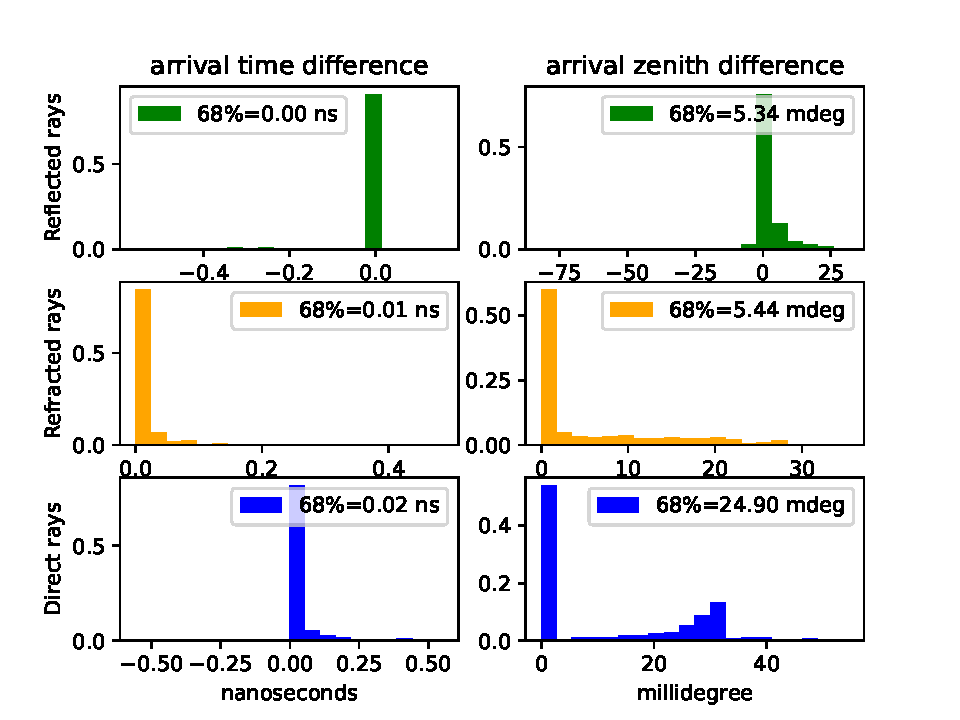
\includegraphics[width=\textwidth]{figures/hybrid_comparison_N_500.pdf}
		\caption{Hybrid}
	\end{figure}
	\end{minipage}
	\begin{minipage}{0.49\textwidth}
	\begin{figure}
		\centering
		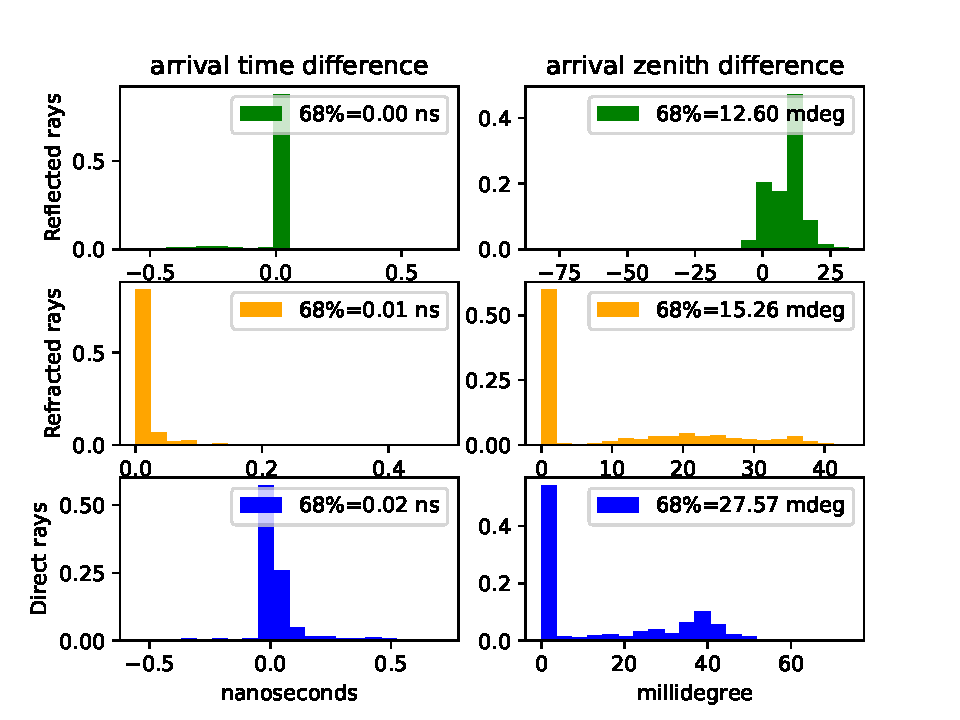
\includegraphics[width=\textwidth]{figures/iterative_comparison_N_500.pdf}
		\caption{Iterative}
	\end{figure}
	\end{minipage}
\end{frame}
\begin{frame}{Why?}
	\begin{itemize}
		\item Complex ice models needed
		\item full path might be needed
	\end{itemize}
\end{frame}

\begin{frame}
	\begin{enumerate}
		\item How the iterative ray tracer works
		\item previous attempt to make it better
		\item my attempt to make it better
		\item optimisation of my attempt (the hybrid raytracer)
		\item final results
	\end{enumerate}
\end{frame}
\begin{frame}{Iterative ray tracer}
	\begin{figure}
		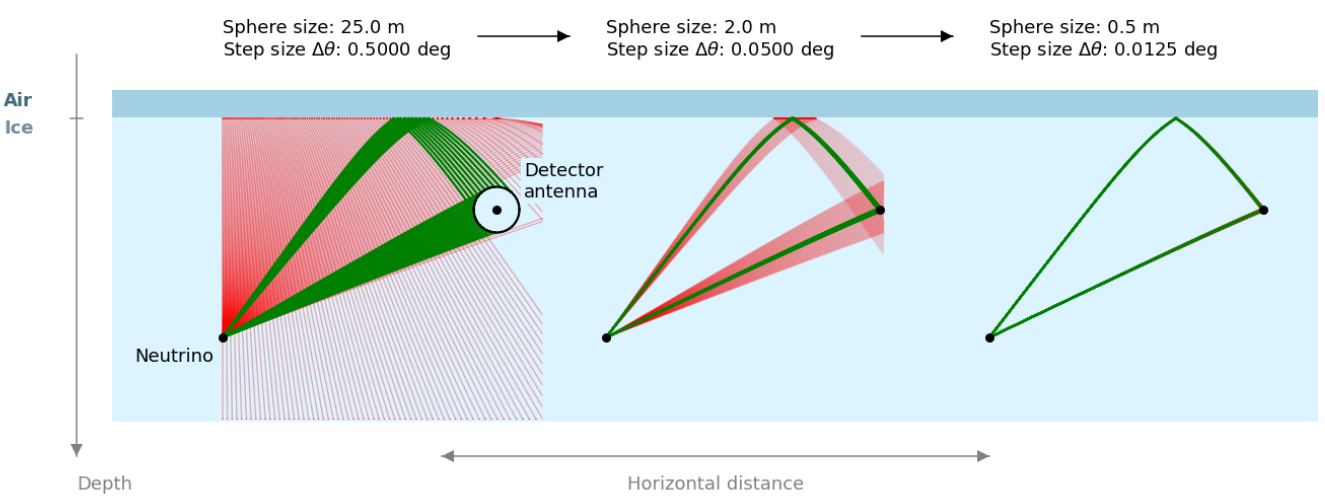
\includegraphics[width=\textwidth]{figures/iterative_explanation.png}
	\end{figure}
\end{frame}
\begin{frame}
	\centering
	Non optimal $\rightarrow$ scipy.optimize.minimize\\\vspace{1cm}
	$\implies$ minimizer
\end{frame}
\begin{frame}
	\begin{figure}
		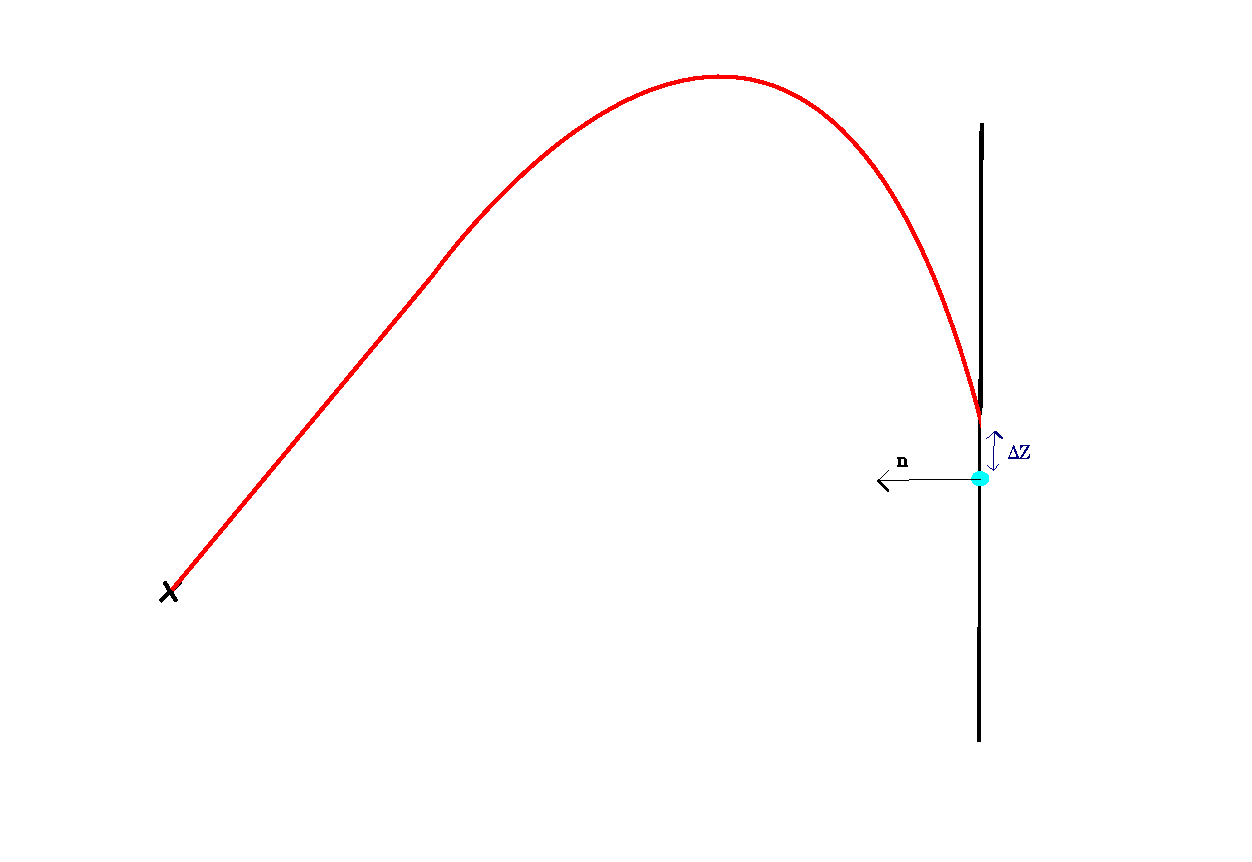
\includegraphics[width=\textwidth]{figures/PrincipleIllu.pdf}
	\end{figure}
\end{frame}
\begin{frame}
	\centering
	Problem: can't find the intervals for certain cases
\end{frame}
\begin{frame}
	\begin{figure}
		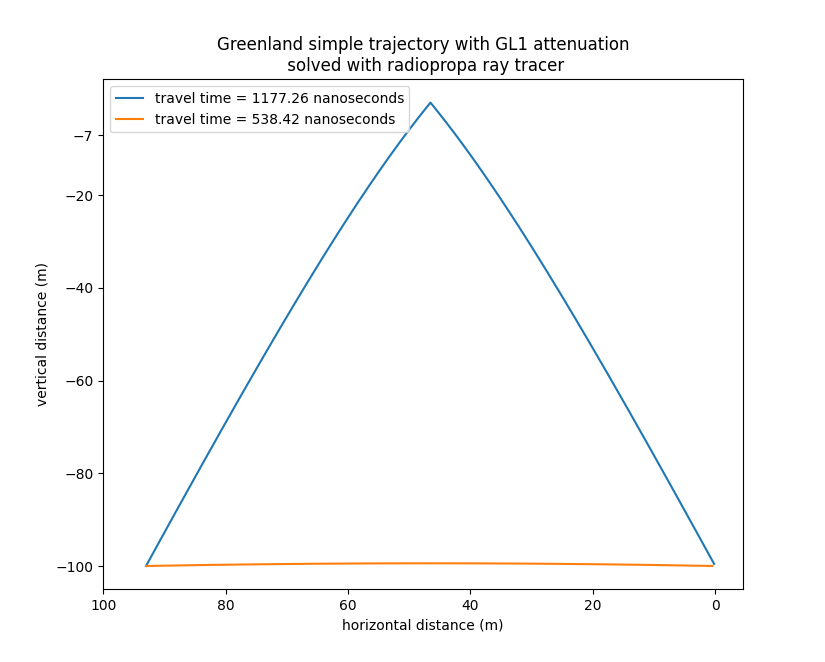
\includegraphics[width=\textwidth]{figures/iterative.png}
	\end{figure}
\end{frame}
\begin{frame}
	\begin{figure}
		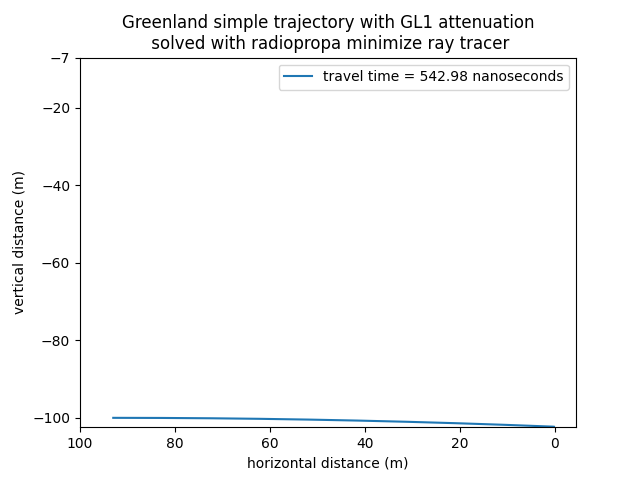
\includegraphics[width=\textwidth]{figures/minimize.png}
	\end{figure}
\end{frame}
\begin{frame}
	\centering
	My solution
\end{frame}
\begin{frame}
	\begin{figure}
		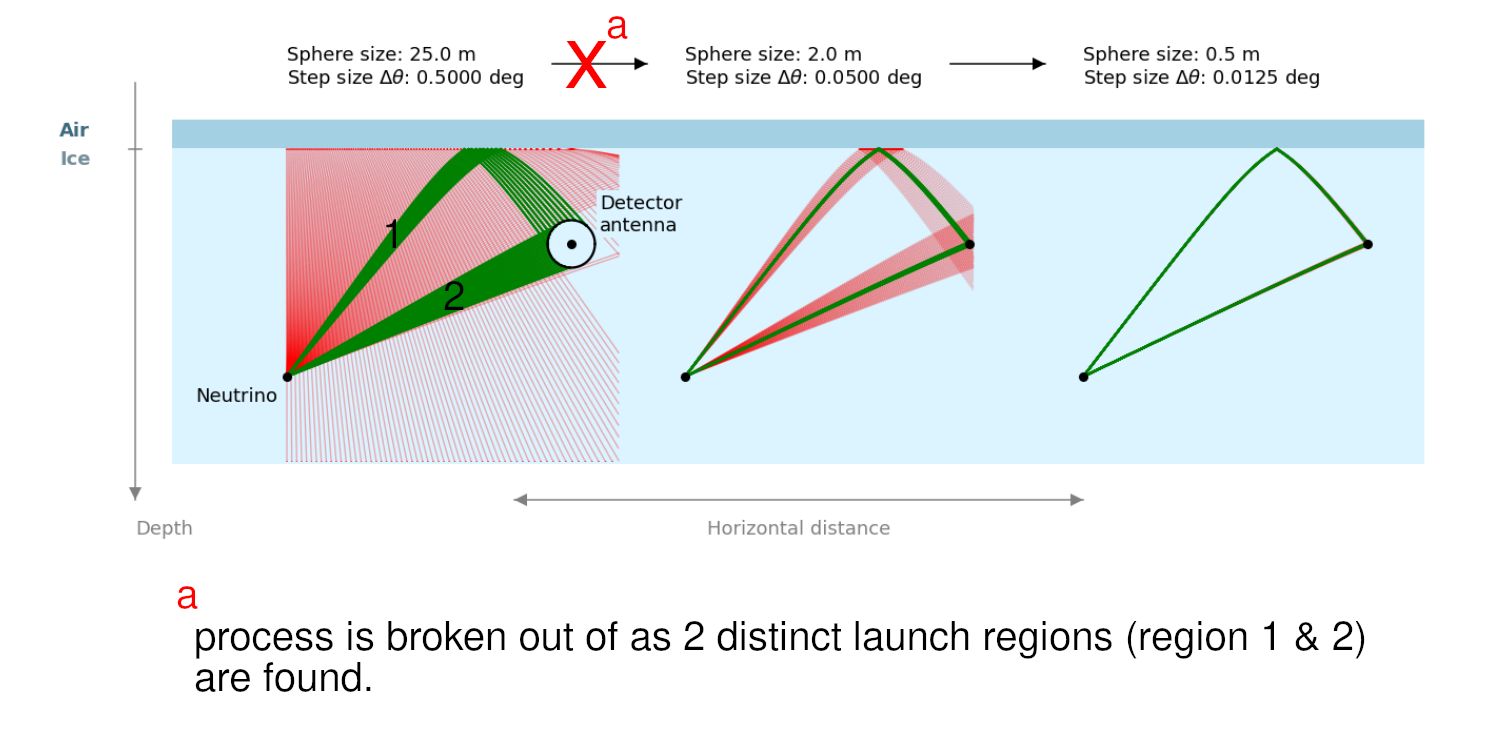
\includegraphics[width=\textwidth]{figures/explanation.png}
	\end{figure}
\end{frame}
\begin{frame}
	\begin{figure}
		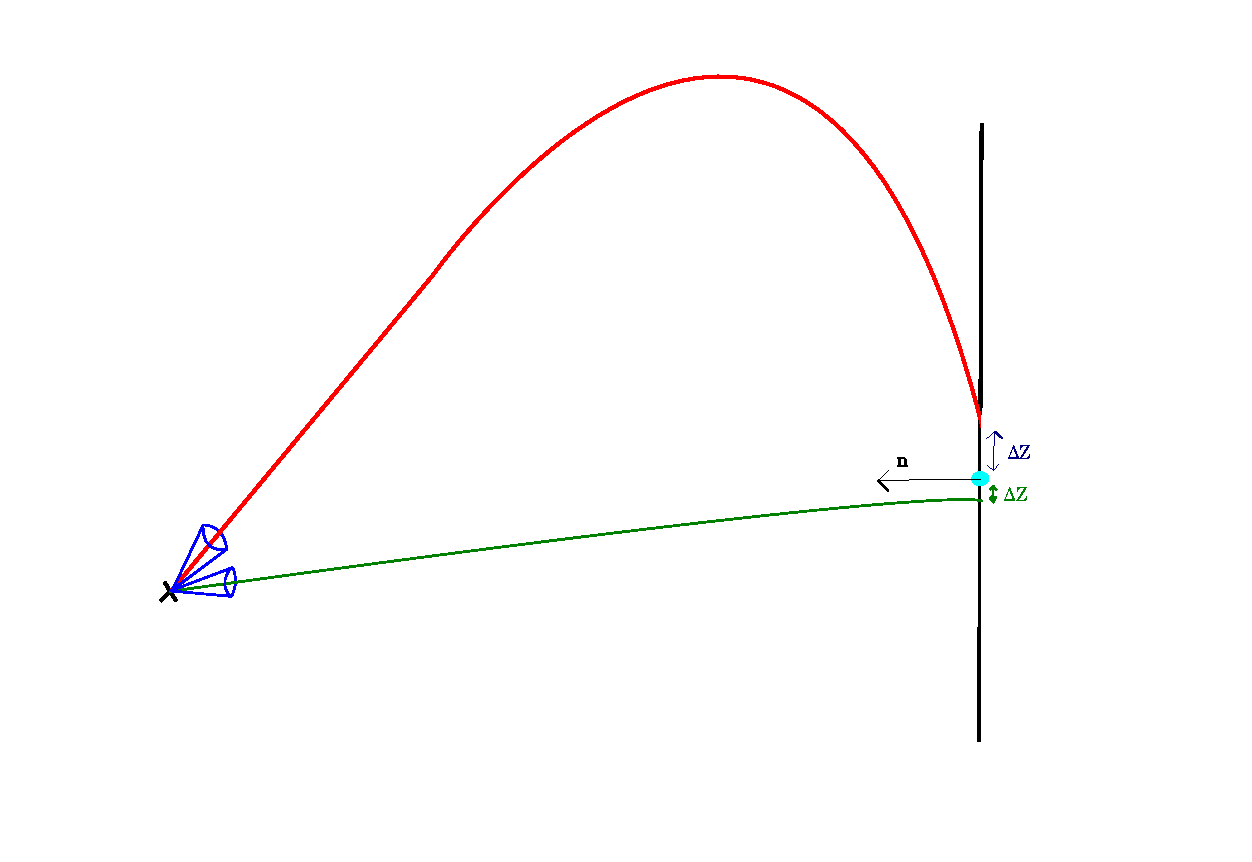
\includegraphics[width=\textwidth]{figures/PrincipleHybridIllu.pdf}
	\end{figure}
\end{frame}
\begin{frame}
	\begin{figure}
		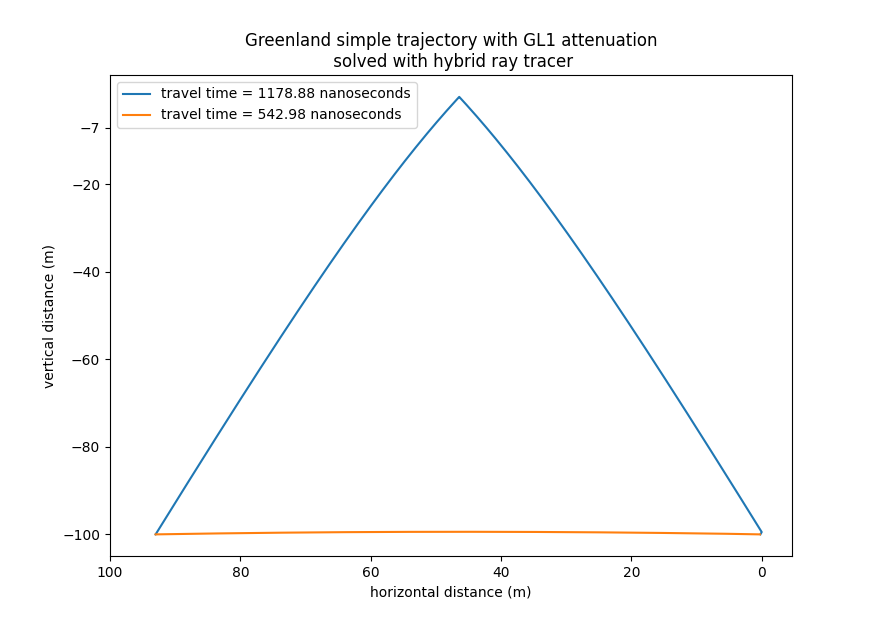
\includegraphics[width=\textwidth]{figures/hybrid.png}
	\end{figure}
\end{frame}
\begin{frame}
	\begin{minipage}{0.49\textwidth}
	\begin{figure}
		\centering
		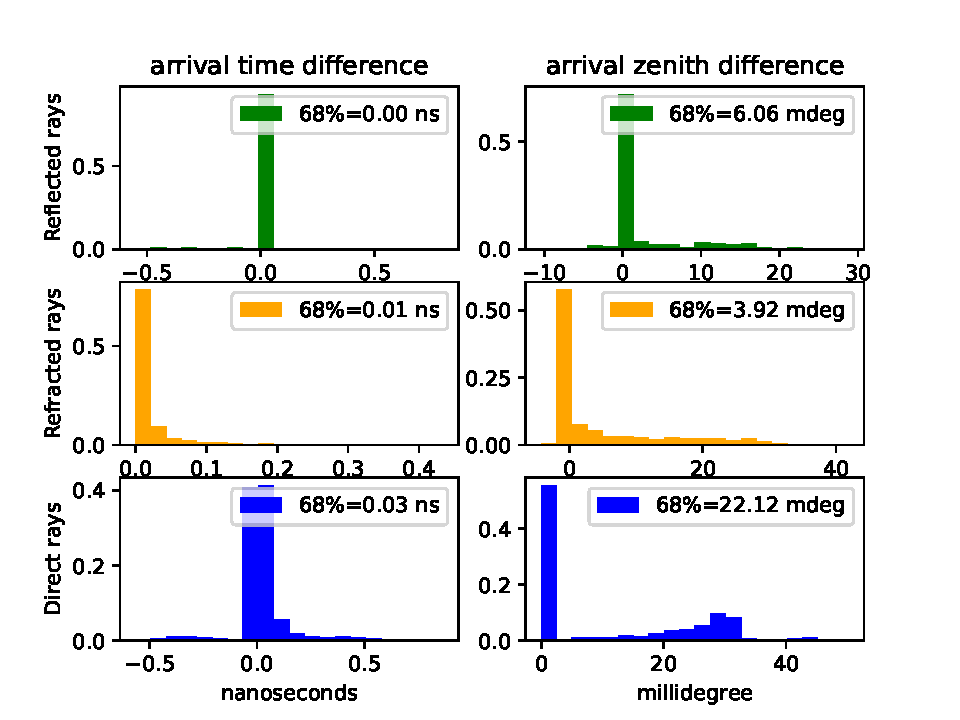
\includegraphics[width=\textwidth]{figures/hybrid_comparison_N_1000.pdf}
		\caption{Hybrid}
	\end{figure}
	\end{minipage}
	\begin{minipage}{0.49\textwidth}
	\begin{figure}
		\centering
		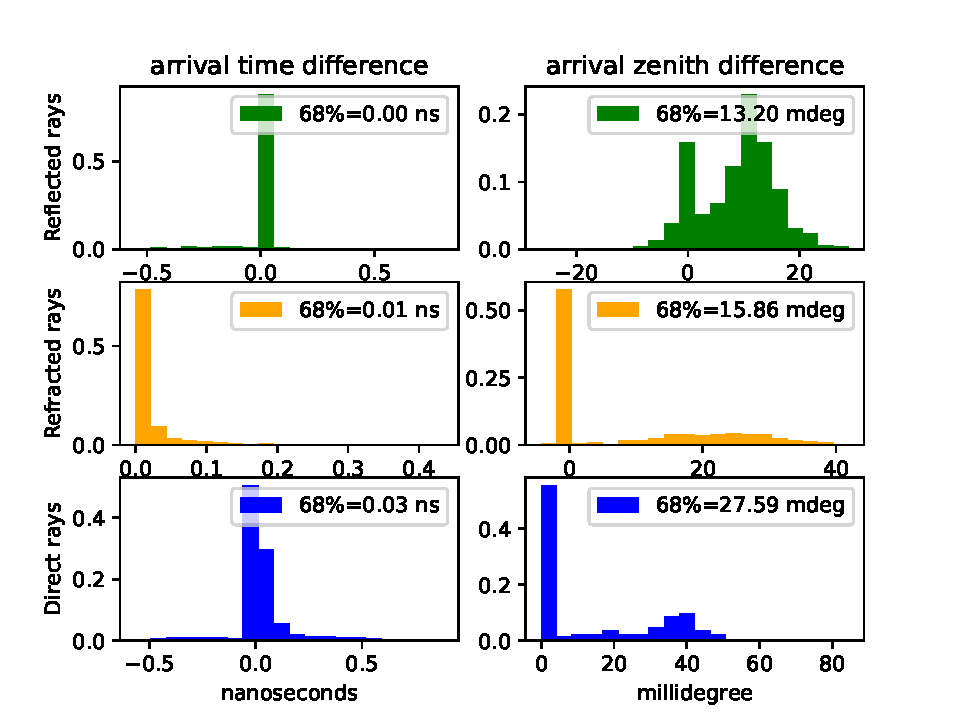
\includegraphics[width=\textwidth]{figures/iterative_comparison_N_1000.pdf}
		\caption{Iterative}
	\end{figure}
	\end{minipage}
Whilst $\approx 15\%$ faster
\end{frame}
\begin{frame}
	\centering
	Optimization
\end{frame}
\begin{frame}
	Length of the normal vector:
	\begin{figure}
		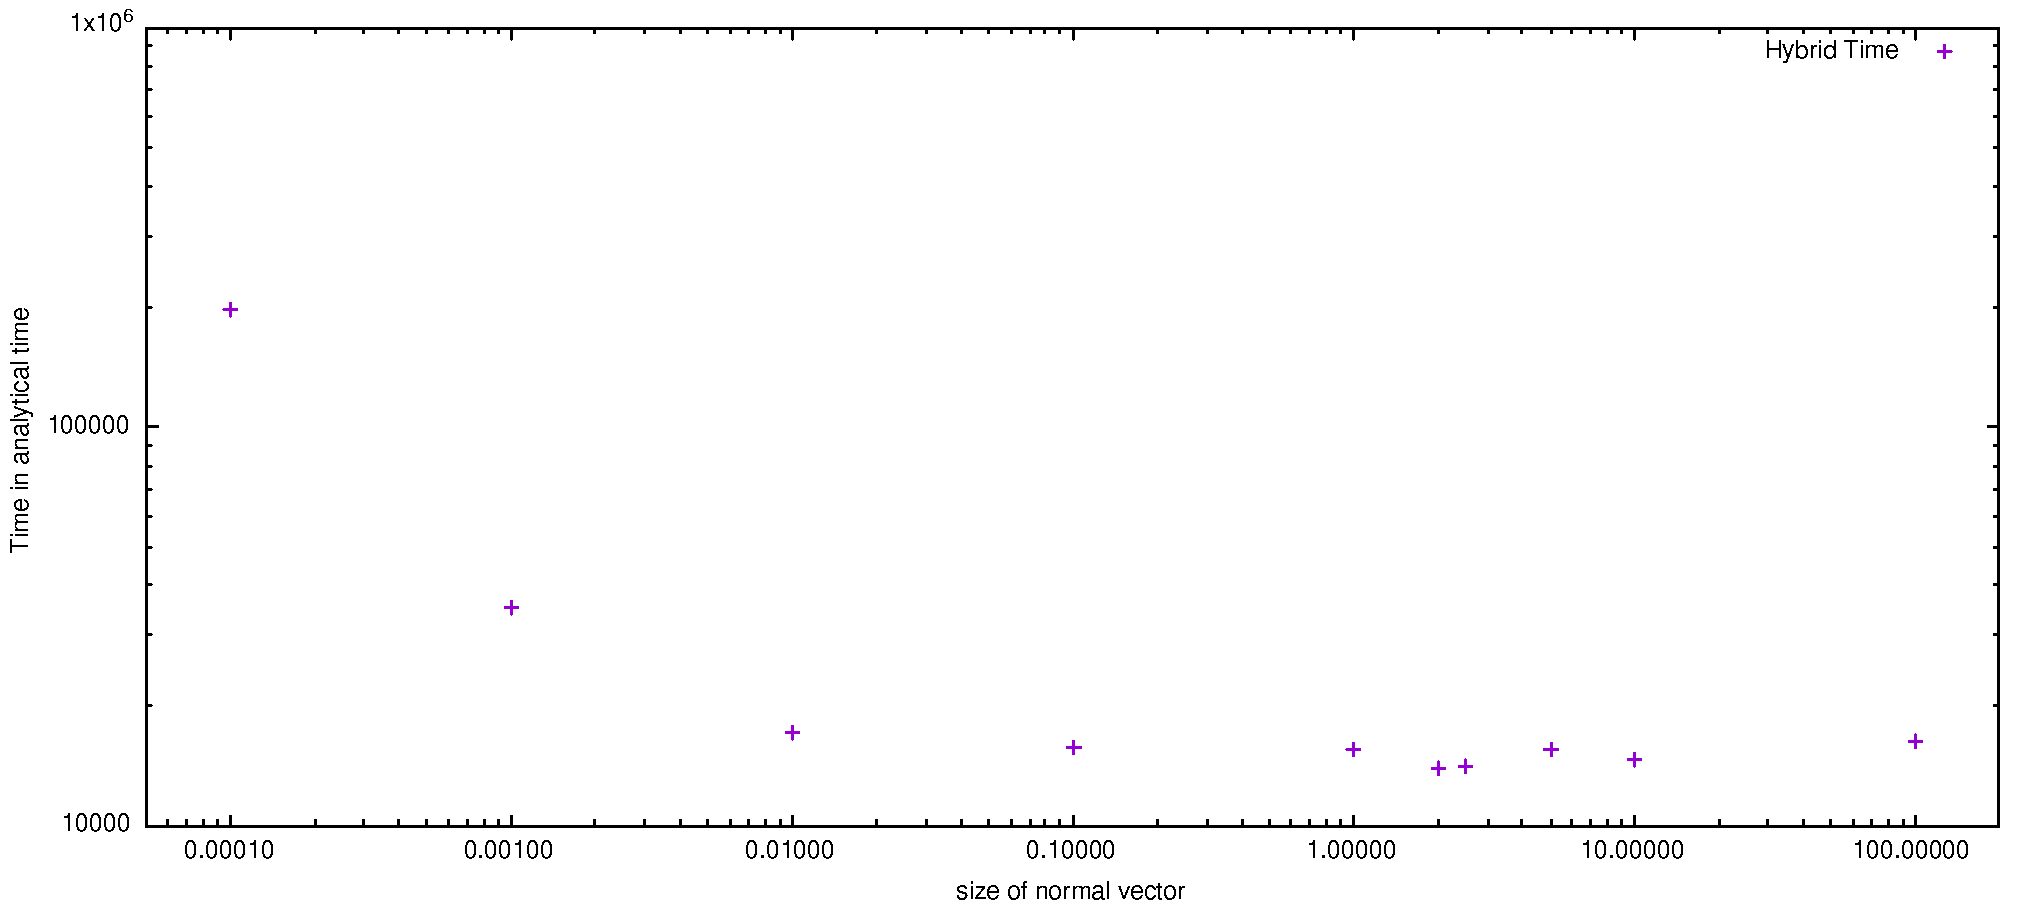
\includegraphics[width=\textwidth]{figures/NormVsRealTime.pdf}
	\end{figure}
\end{frame}
\begin{frame}
	\begin{figure}
		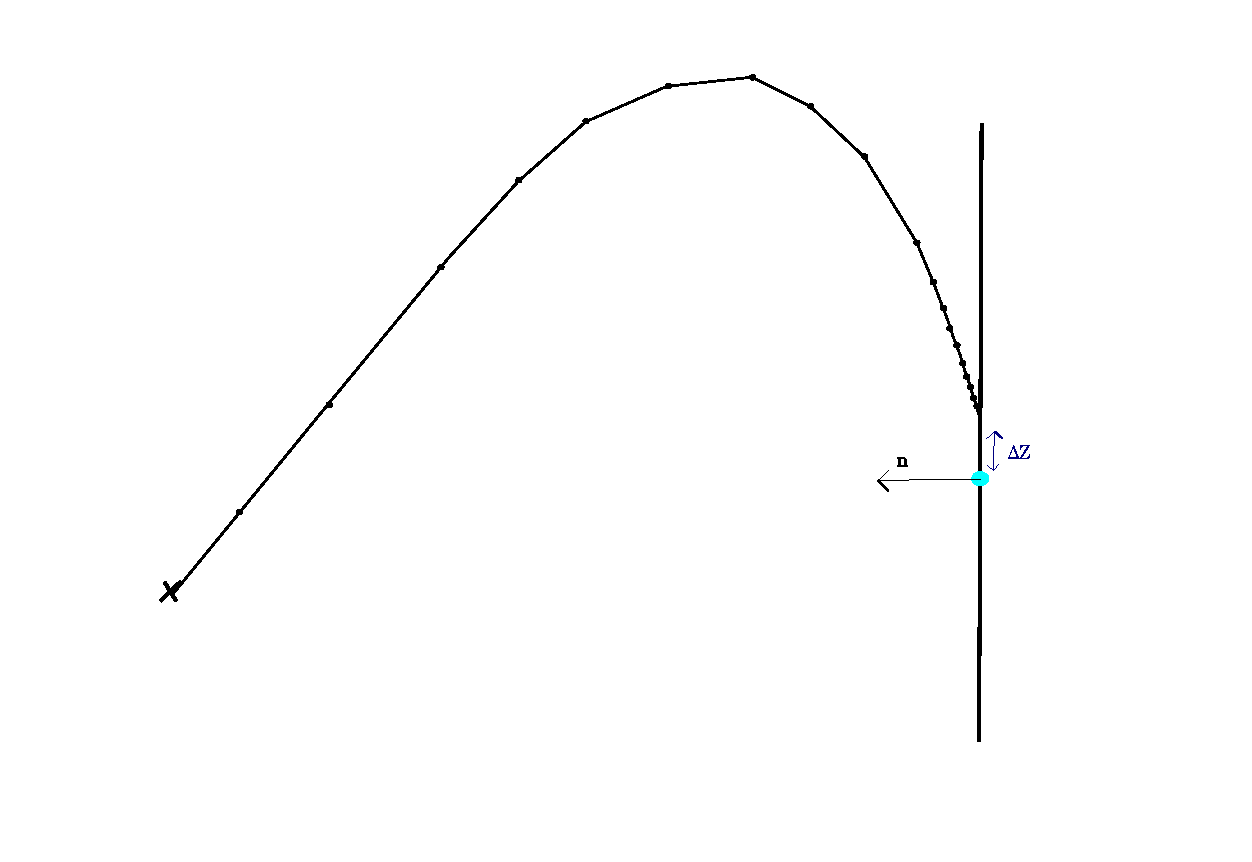
\includegraphics[width=\textwidth]{figures/PrincipleNormIllu.pdf}
	\end{figure}
\end{frame}
\begin{frame}
	\begin{figure}
		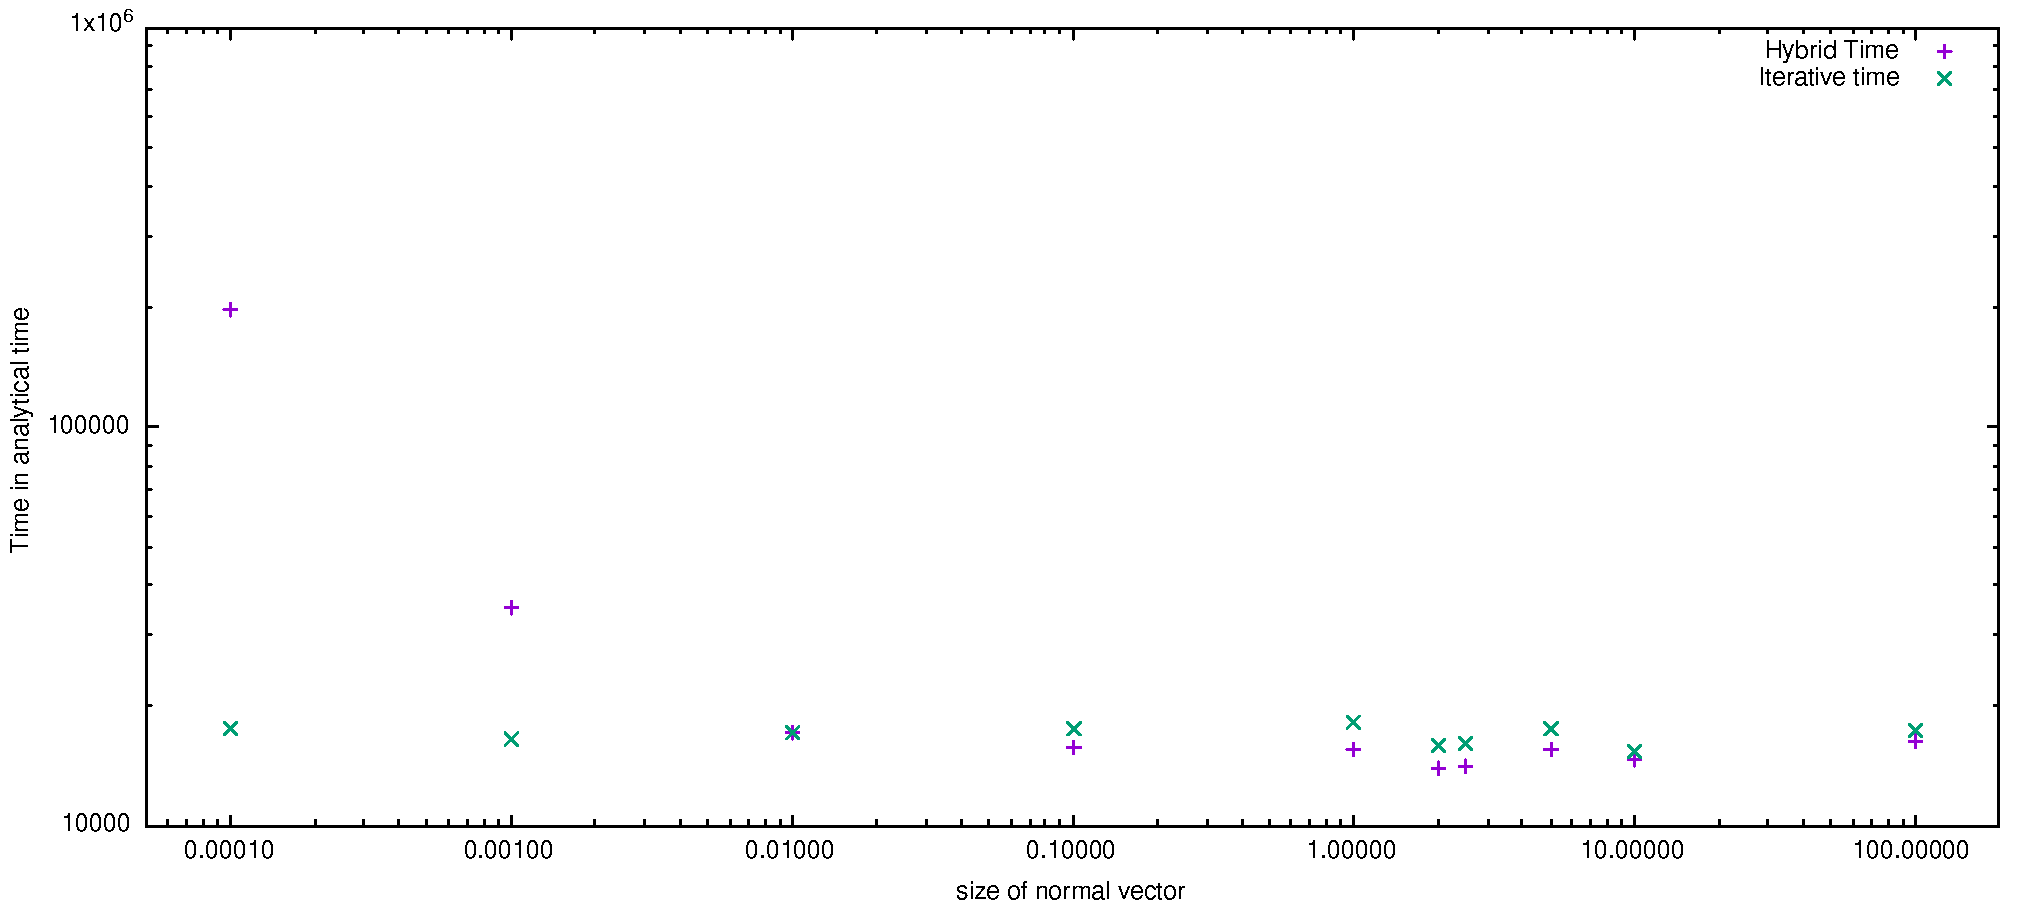
\includegraphics[width=\textwidth]{figures/NormVsRealTime2.pdf}
	\end{figure}
\end{frame}
\begin{frame}
	\begin{figure}
		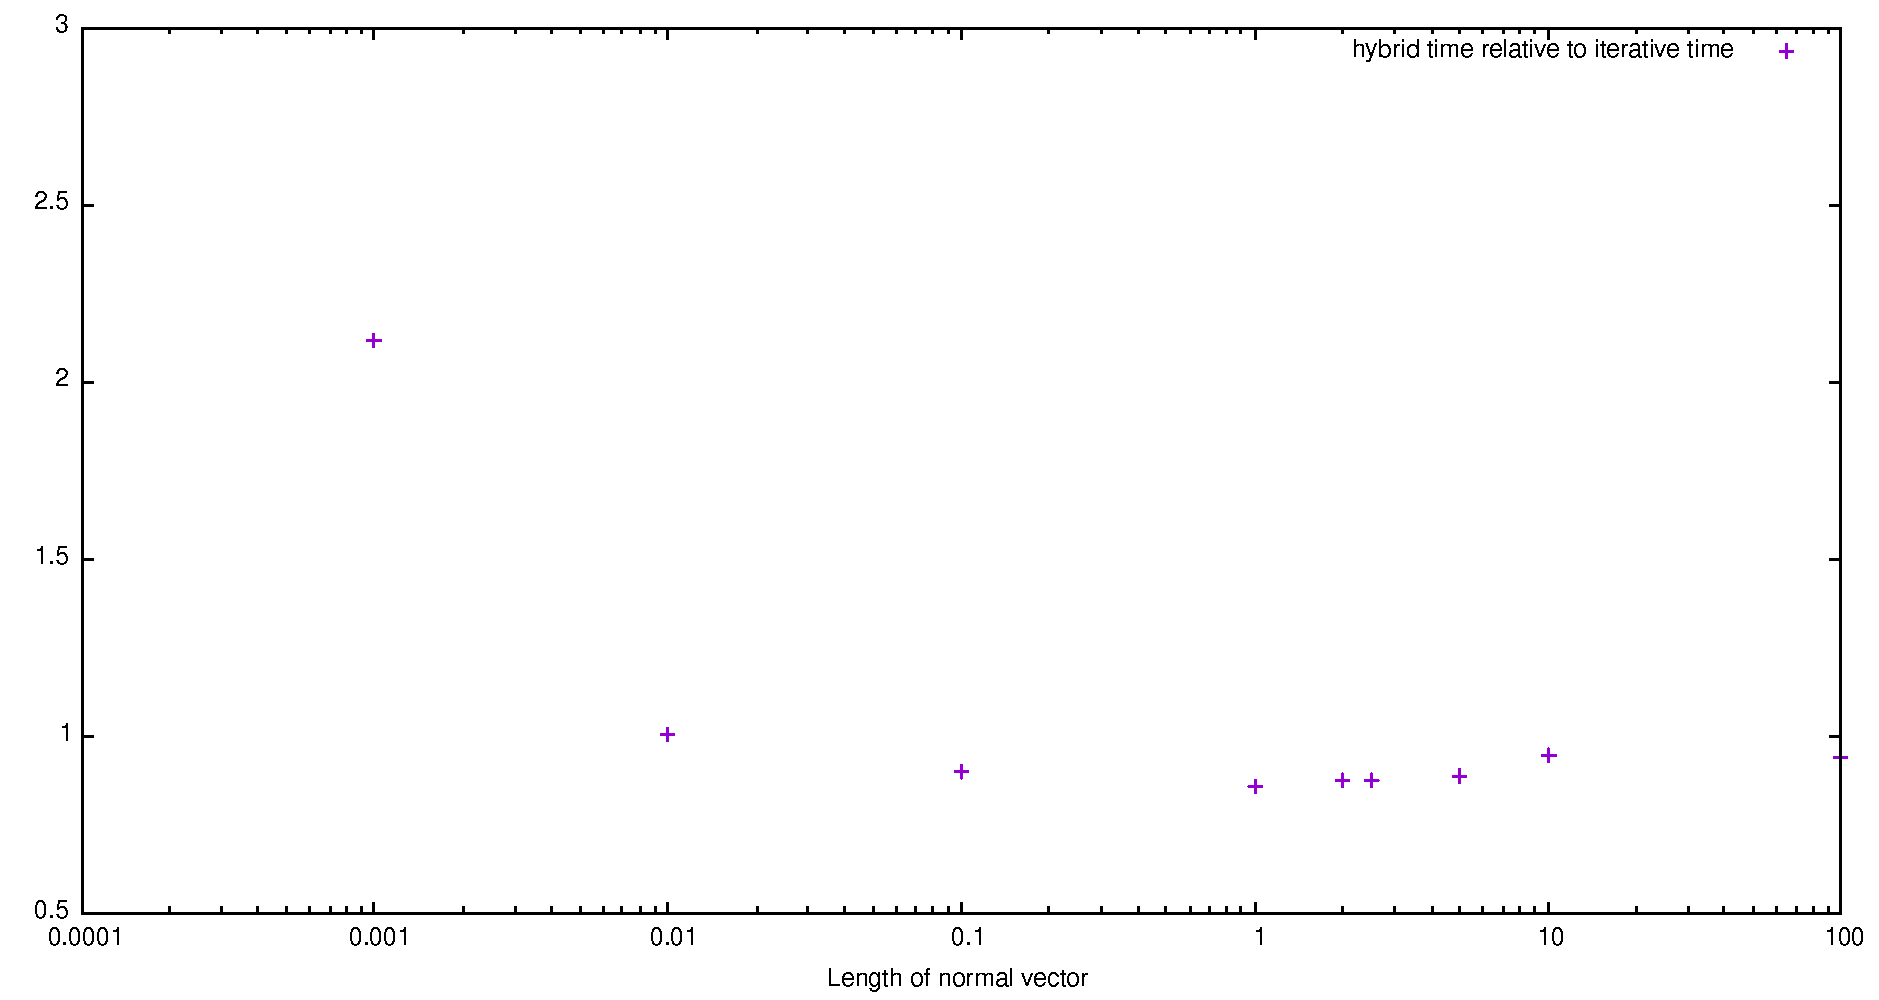
\includegraphics[width=\textwidth]{figures/NormVsTime.pdf}
	\end{figure}
\end{frame}
\begin{frame}
	\begin{figure}
		\begin{minipage}{\textwidth}
			\centering
			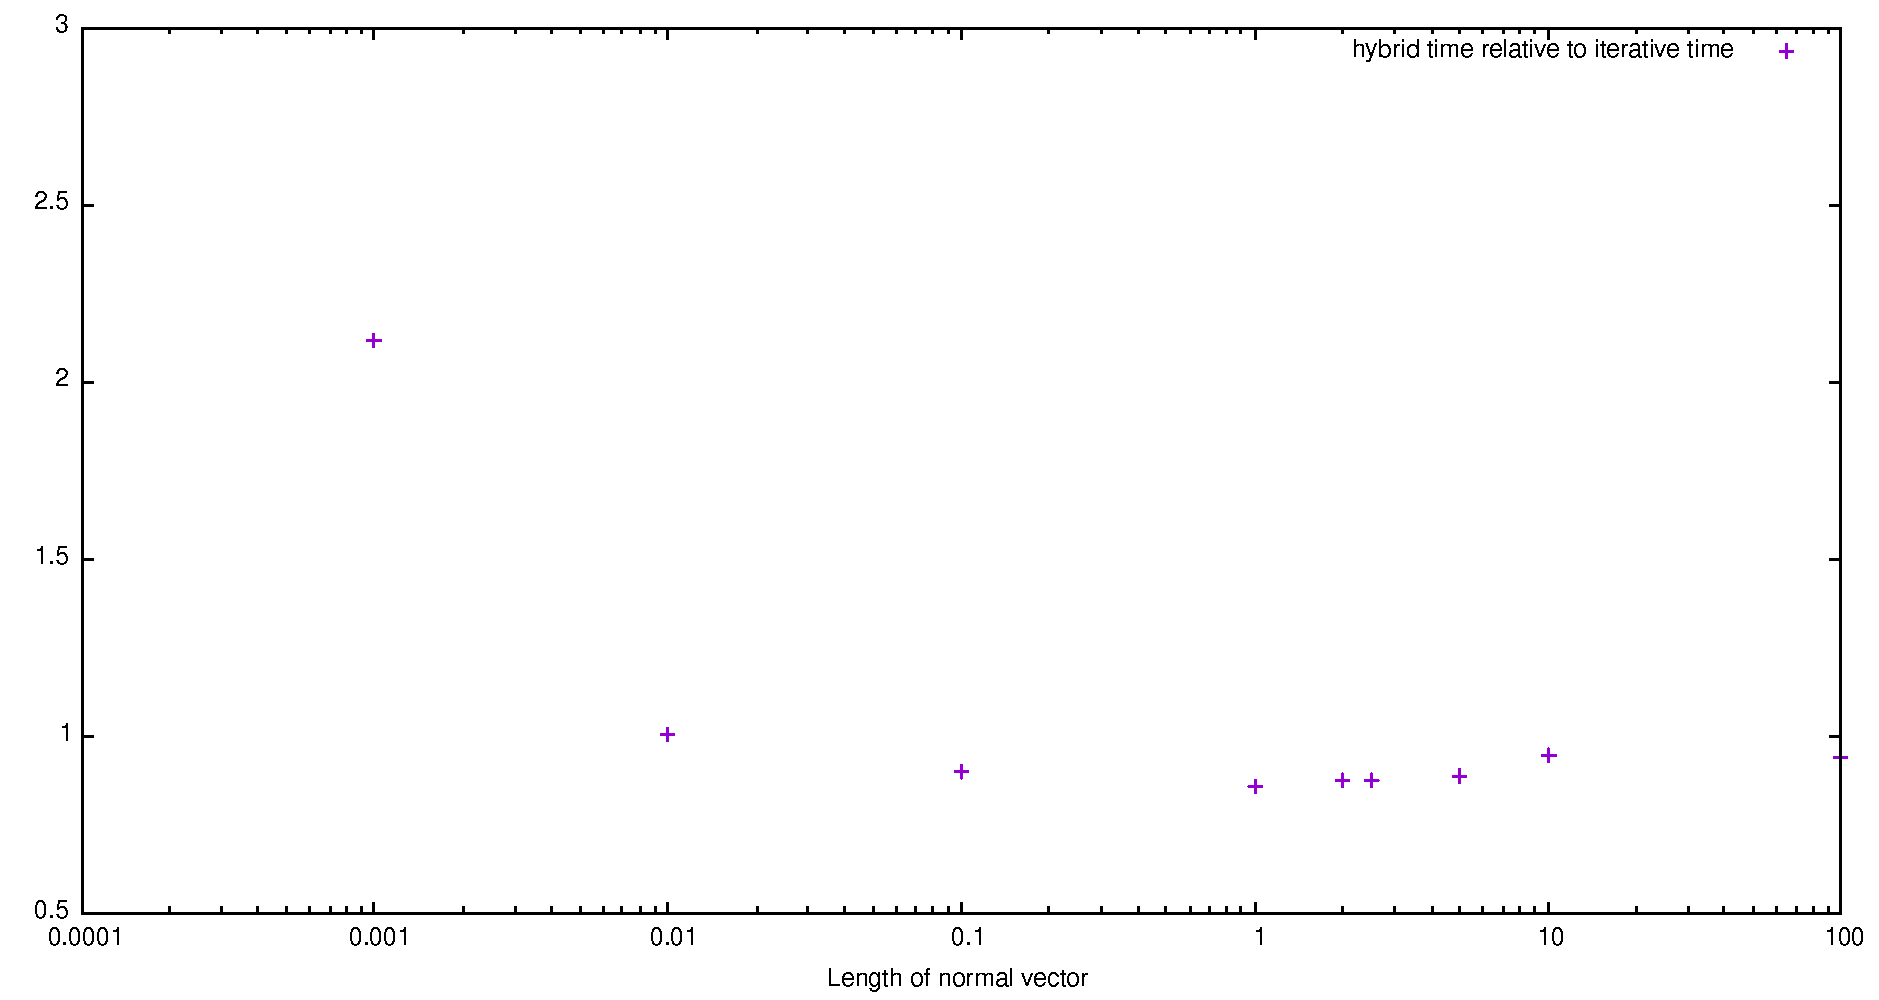
\includegraphics[height=0.45\textheight]{figures/NormVsTime.pdf}
		\end{minipage}
		\begin{minipage}{\textwidth}
			\centering
			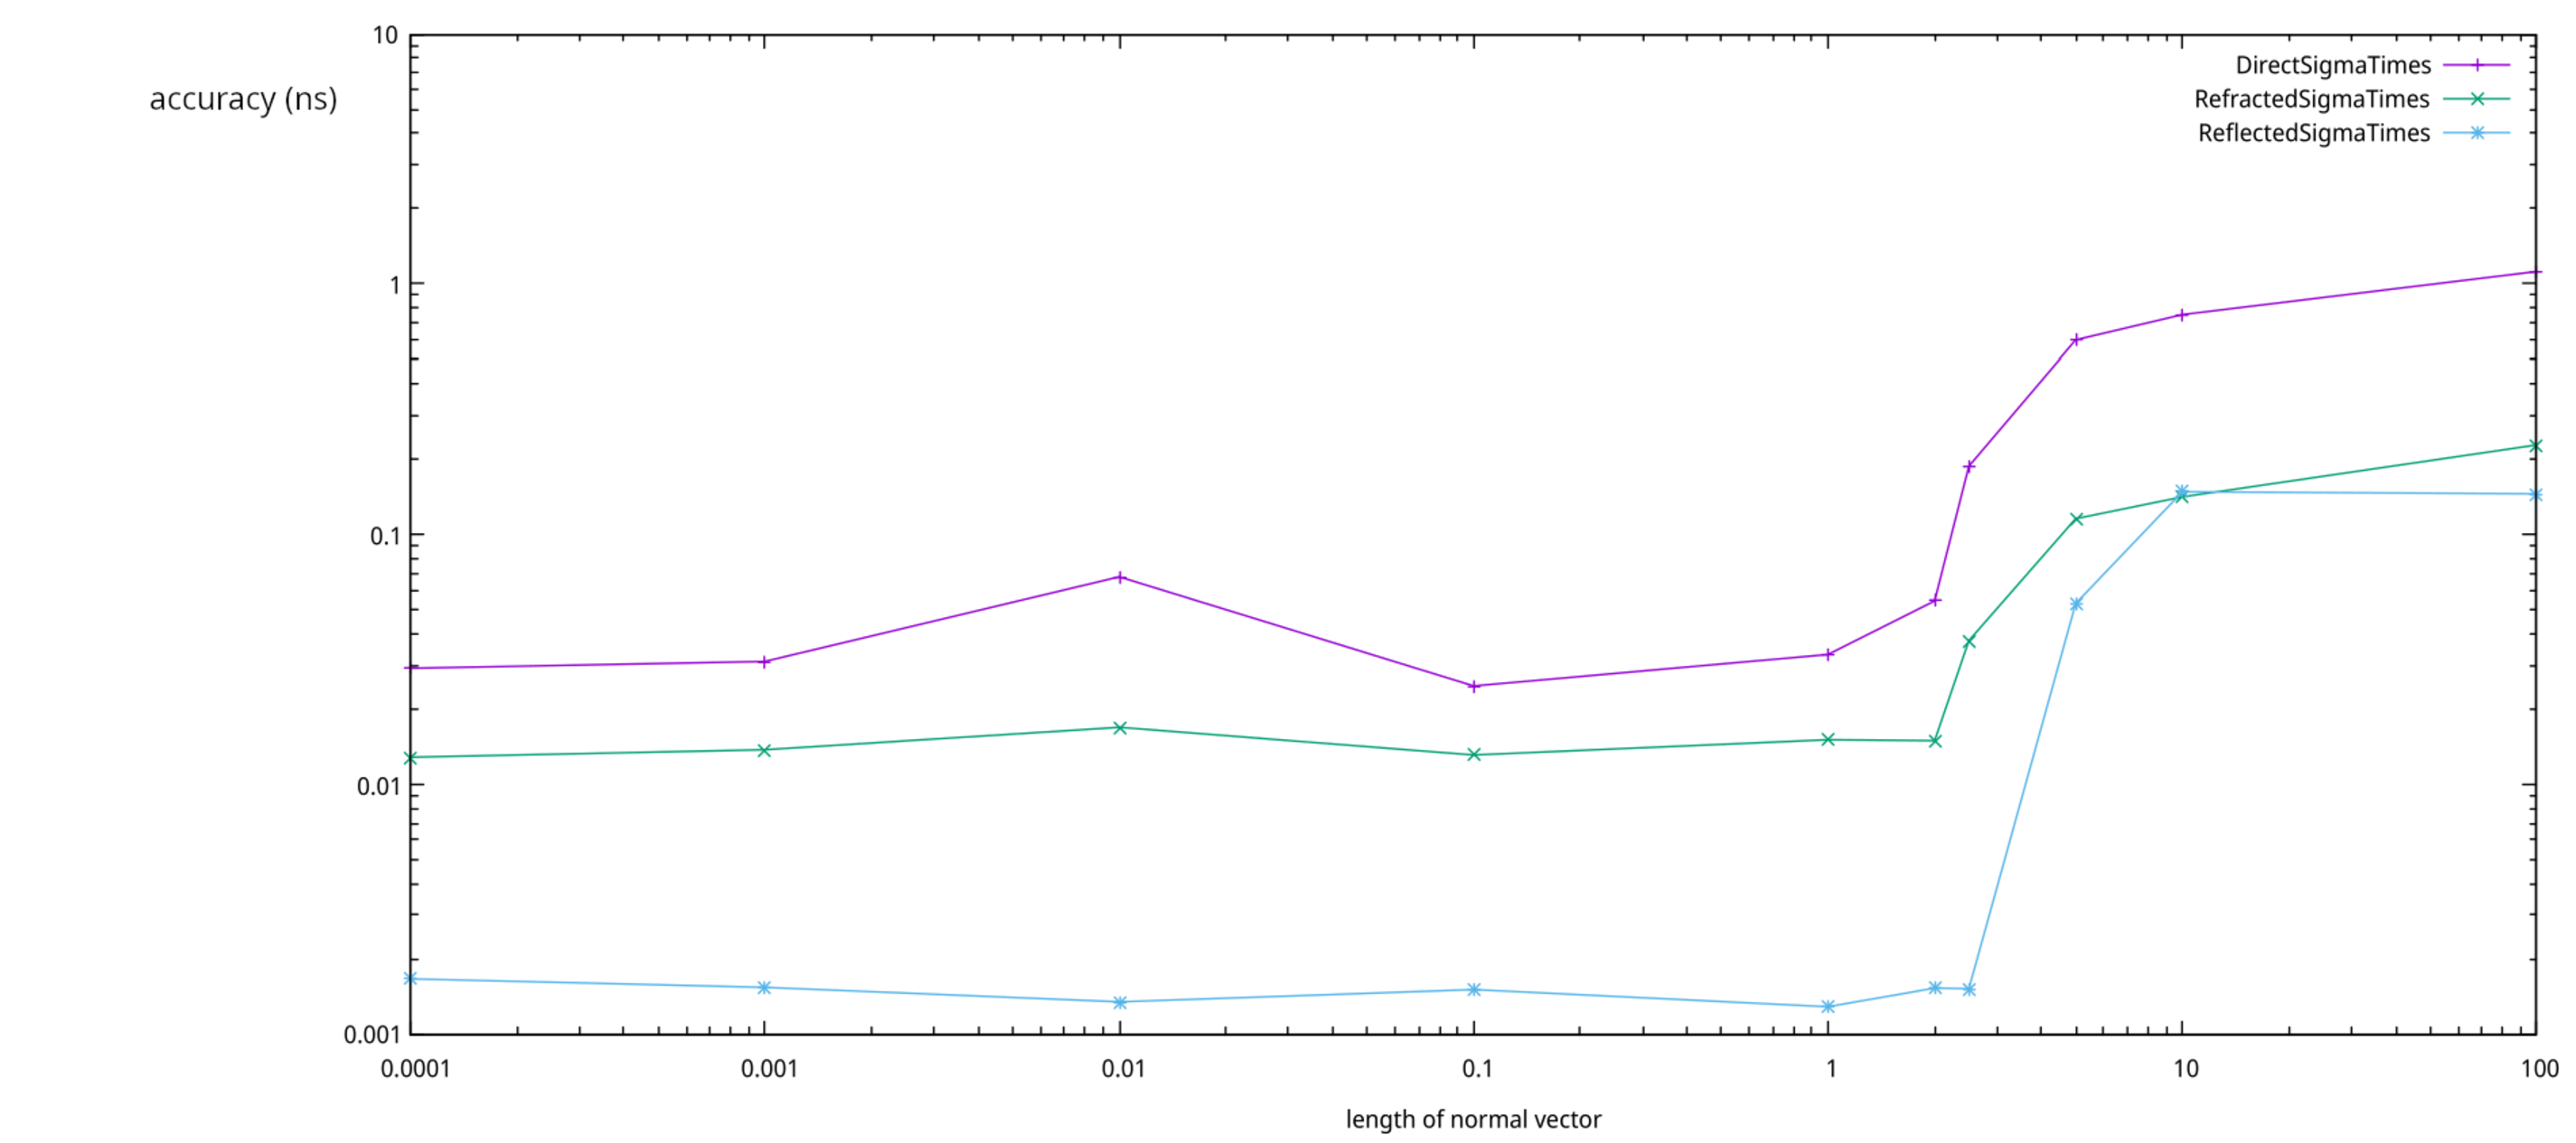
\includegraphics[height=0.45\textheight]{figures/NormVsSigmaTime.pdf}
		\end{minipage}
	\end{figure}
\end{frame}
\begin{frame}
	\begin{figure}
		\begin{minipage}{\textwidth}
			\centering
			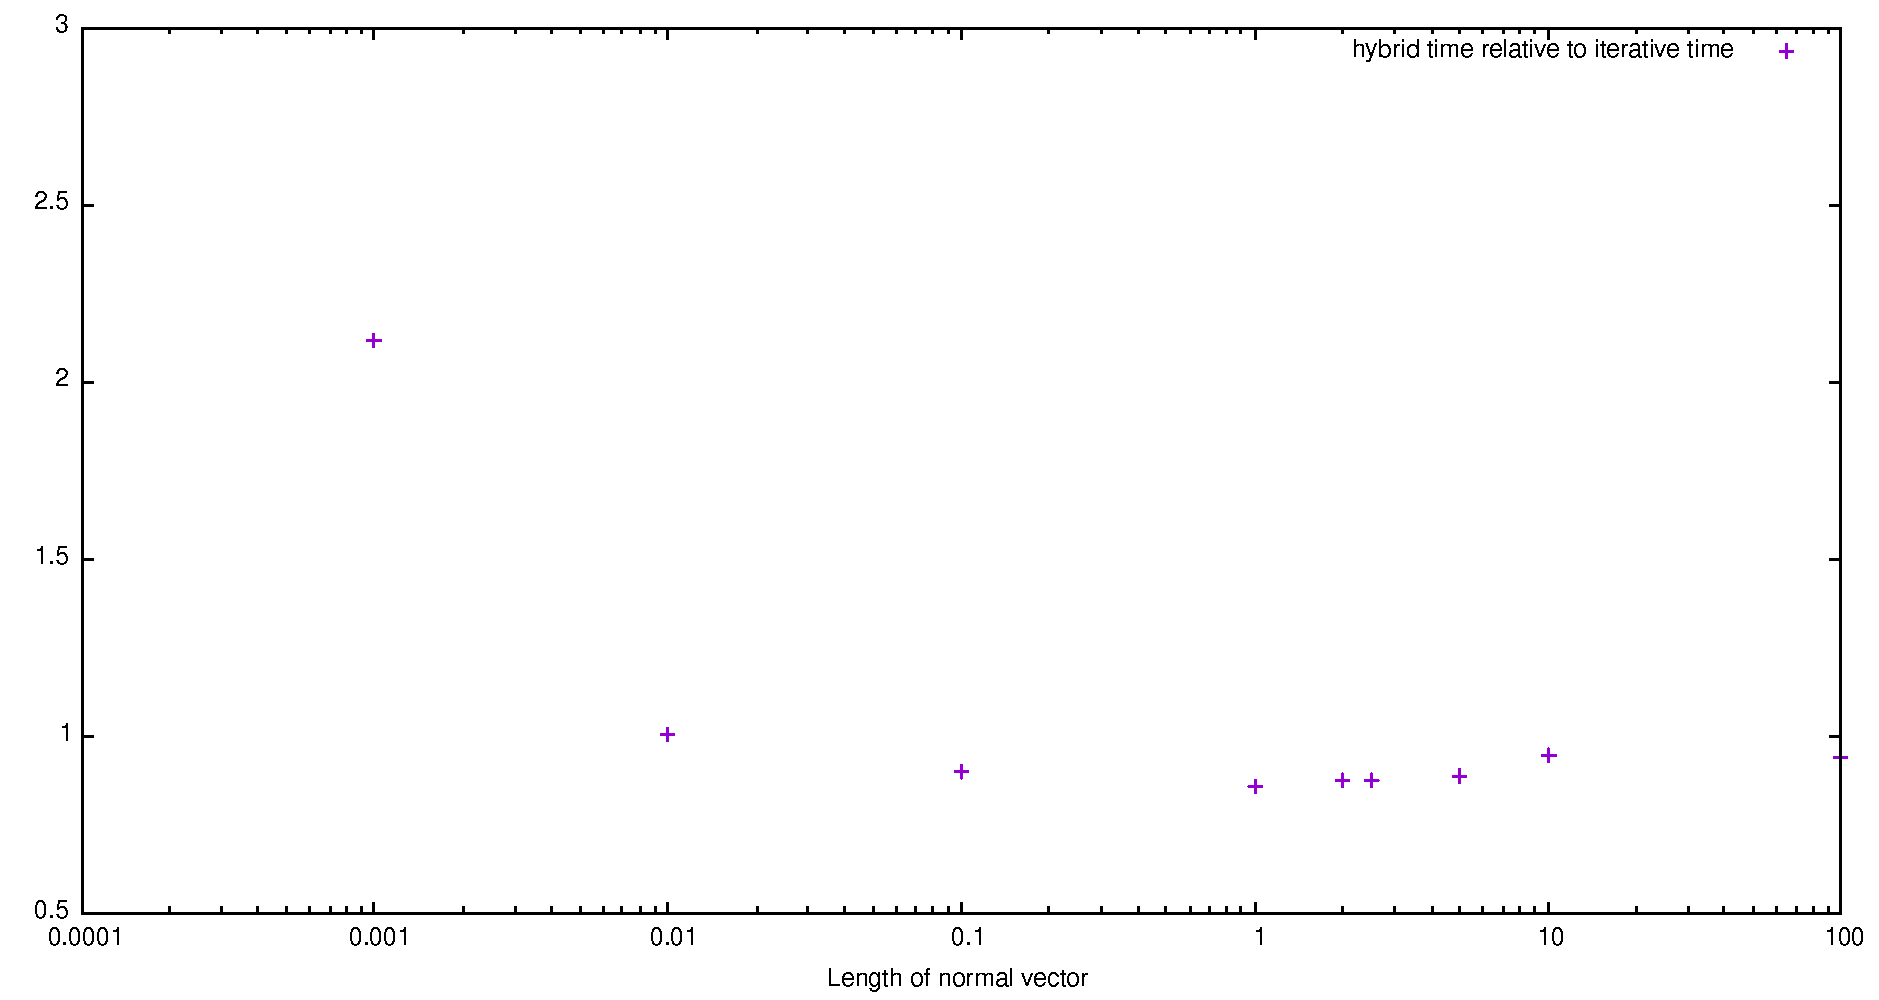
\includegraphics[height=0.45\textheight]{figures/NormVsTime.pdf}
		\end{minipage}
		\begin{minipage}{\textwidth}
			\centering
			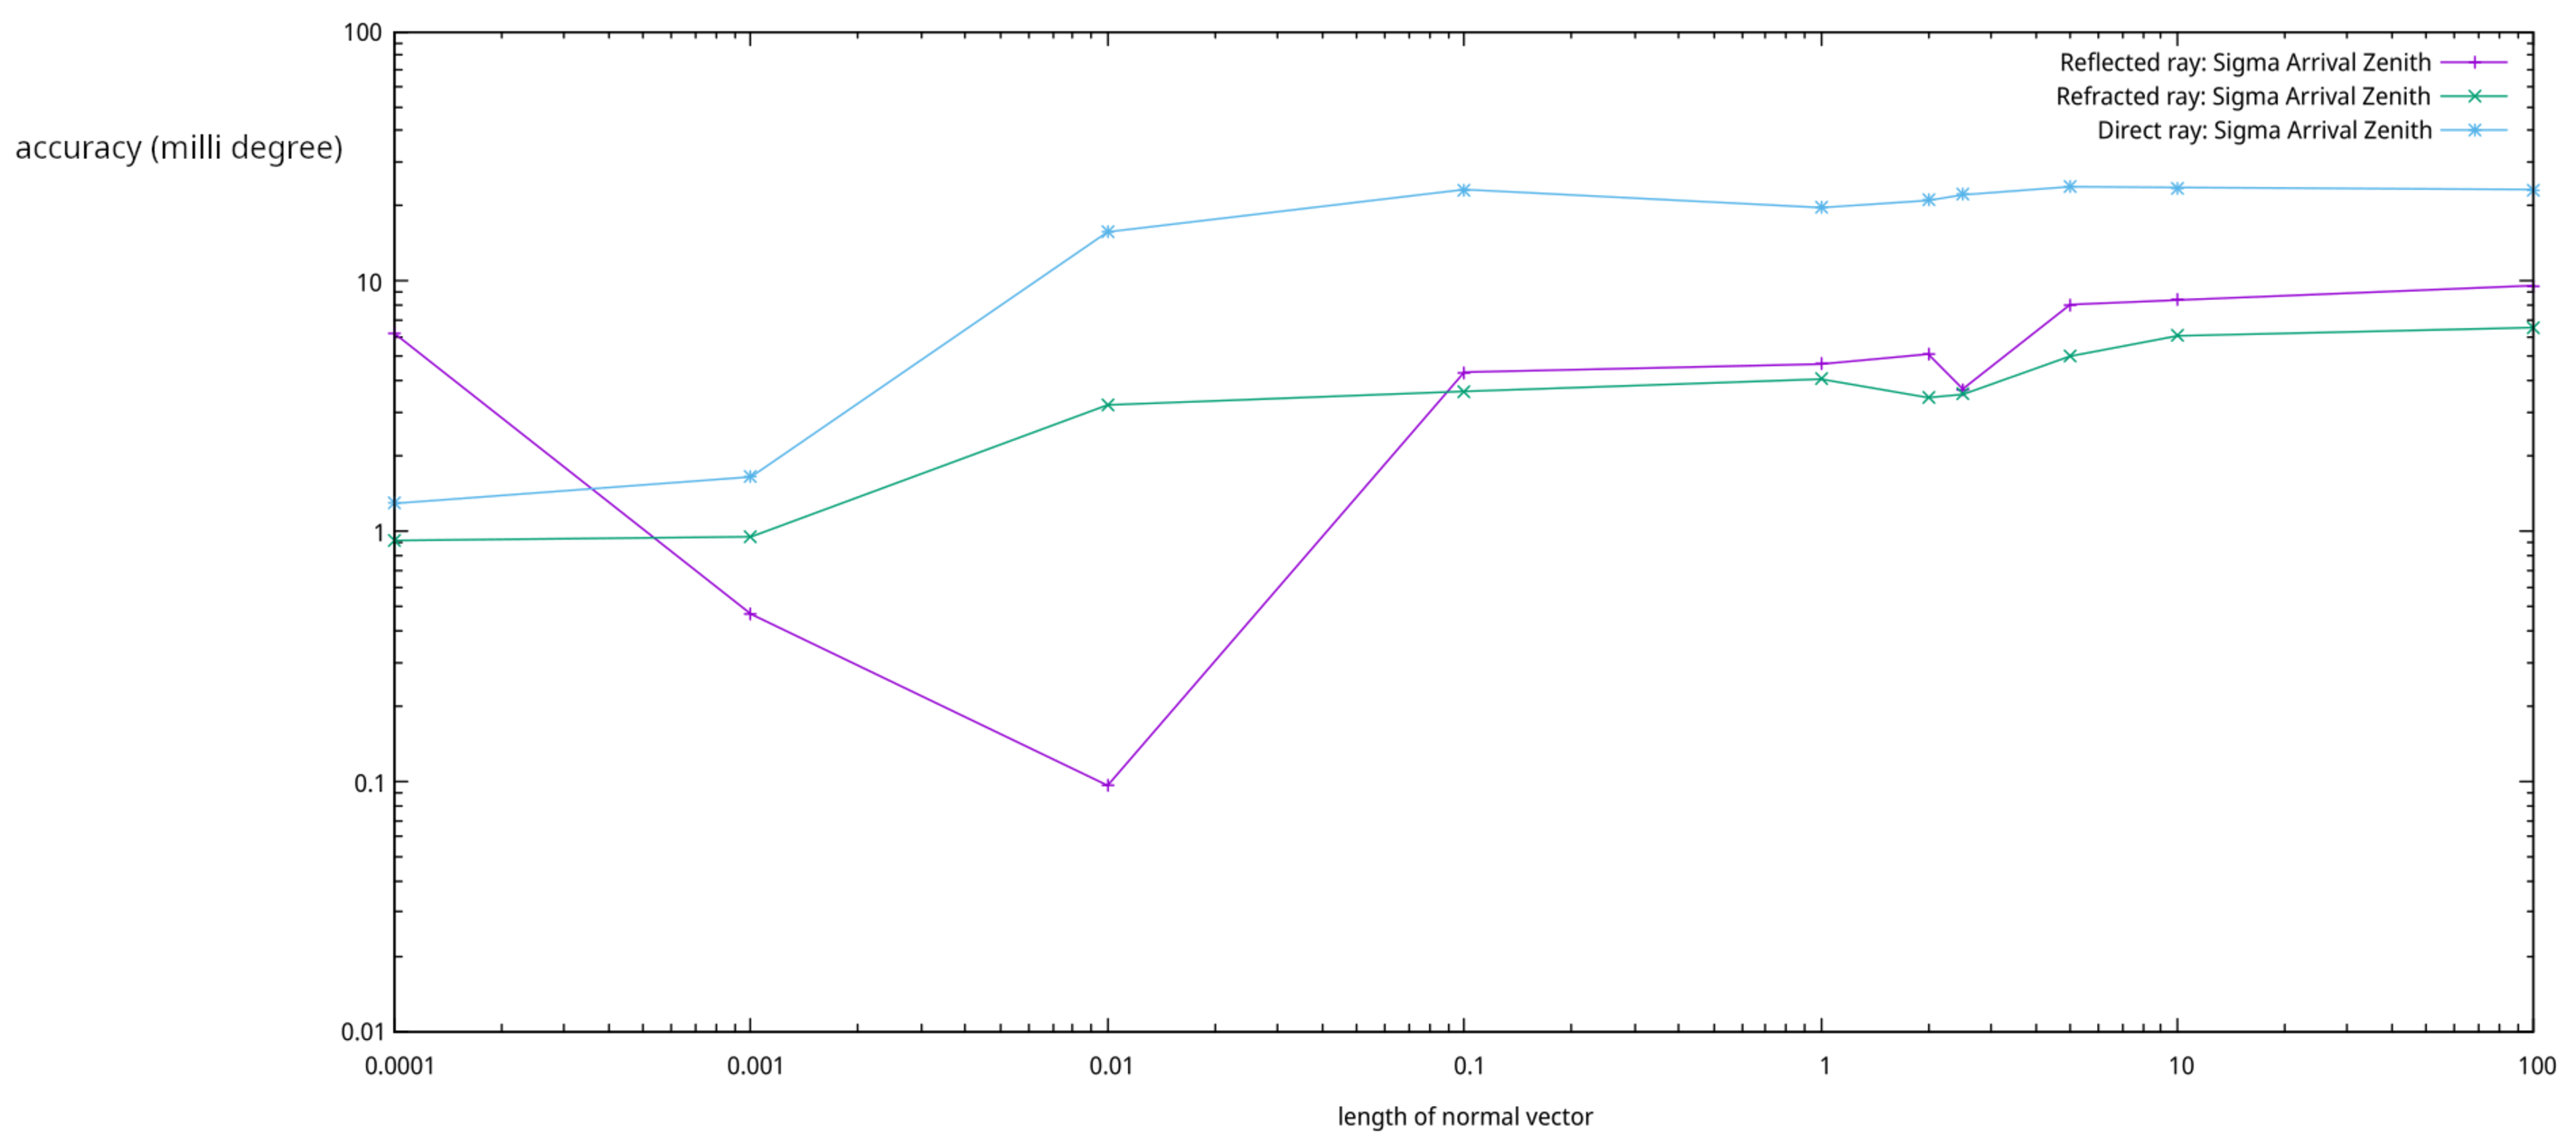
\includegraphics[height=0.45\textheight]{figures/NormVsSigmaAZ.pdf}
		\end{minipage}
	\end{figure}
\end{frame}
\begin{frame}
	\begin{figure}
		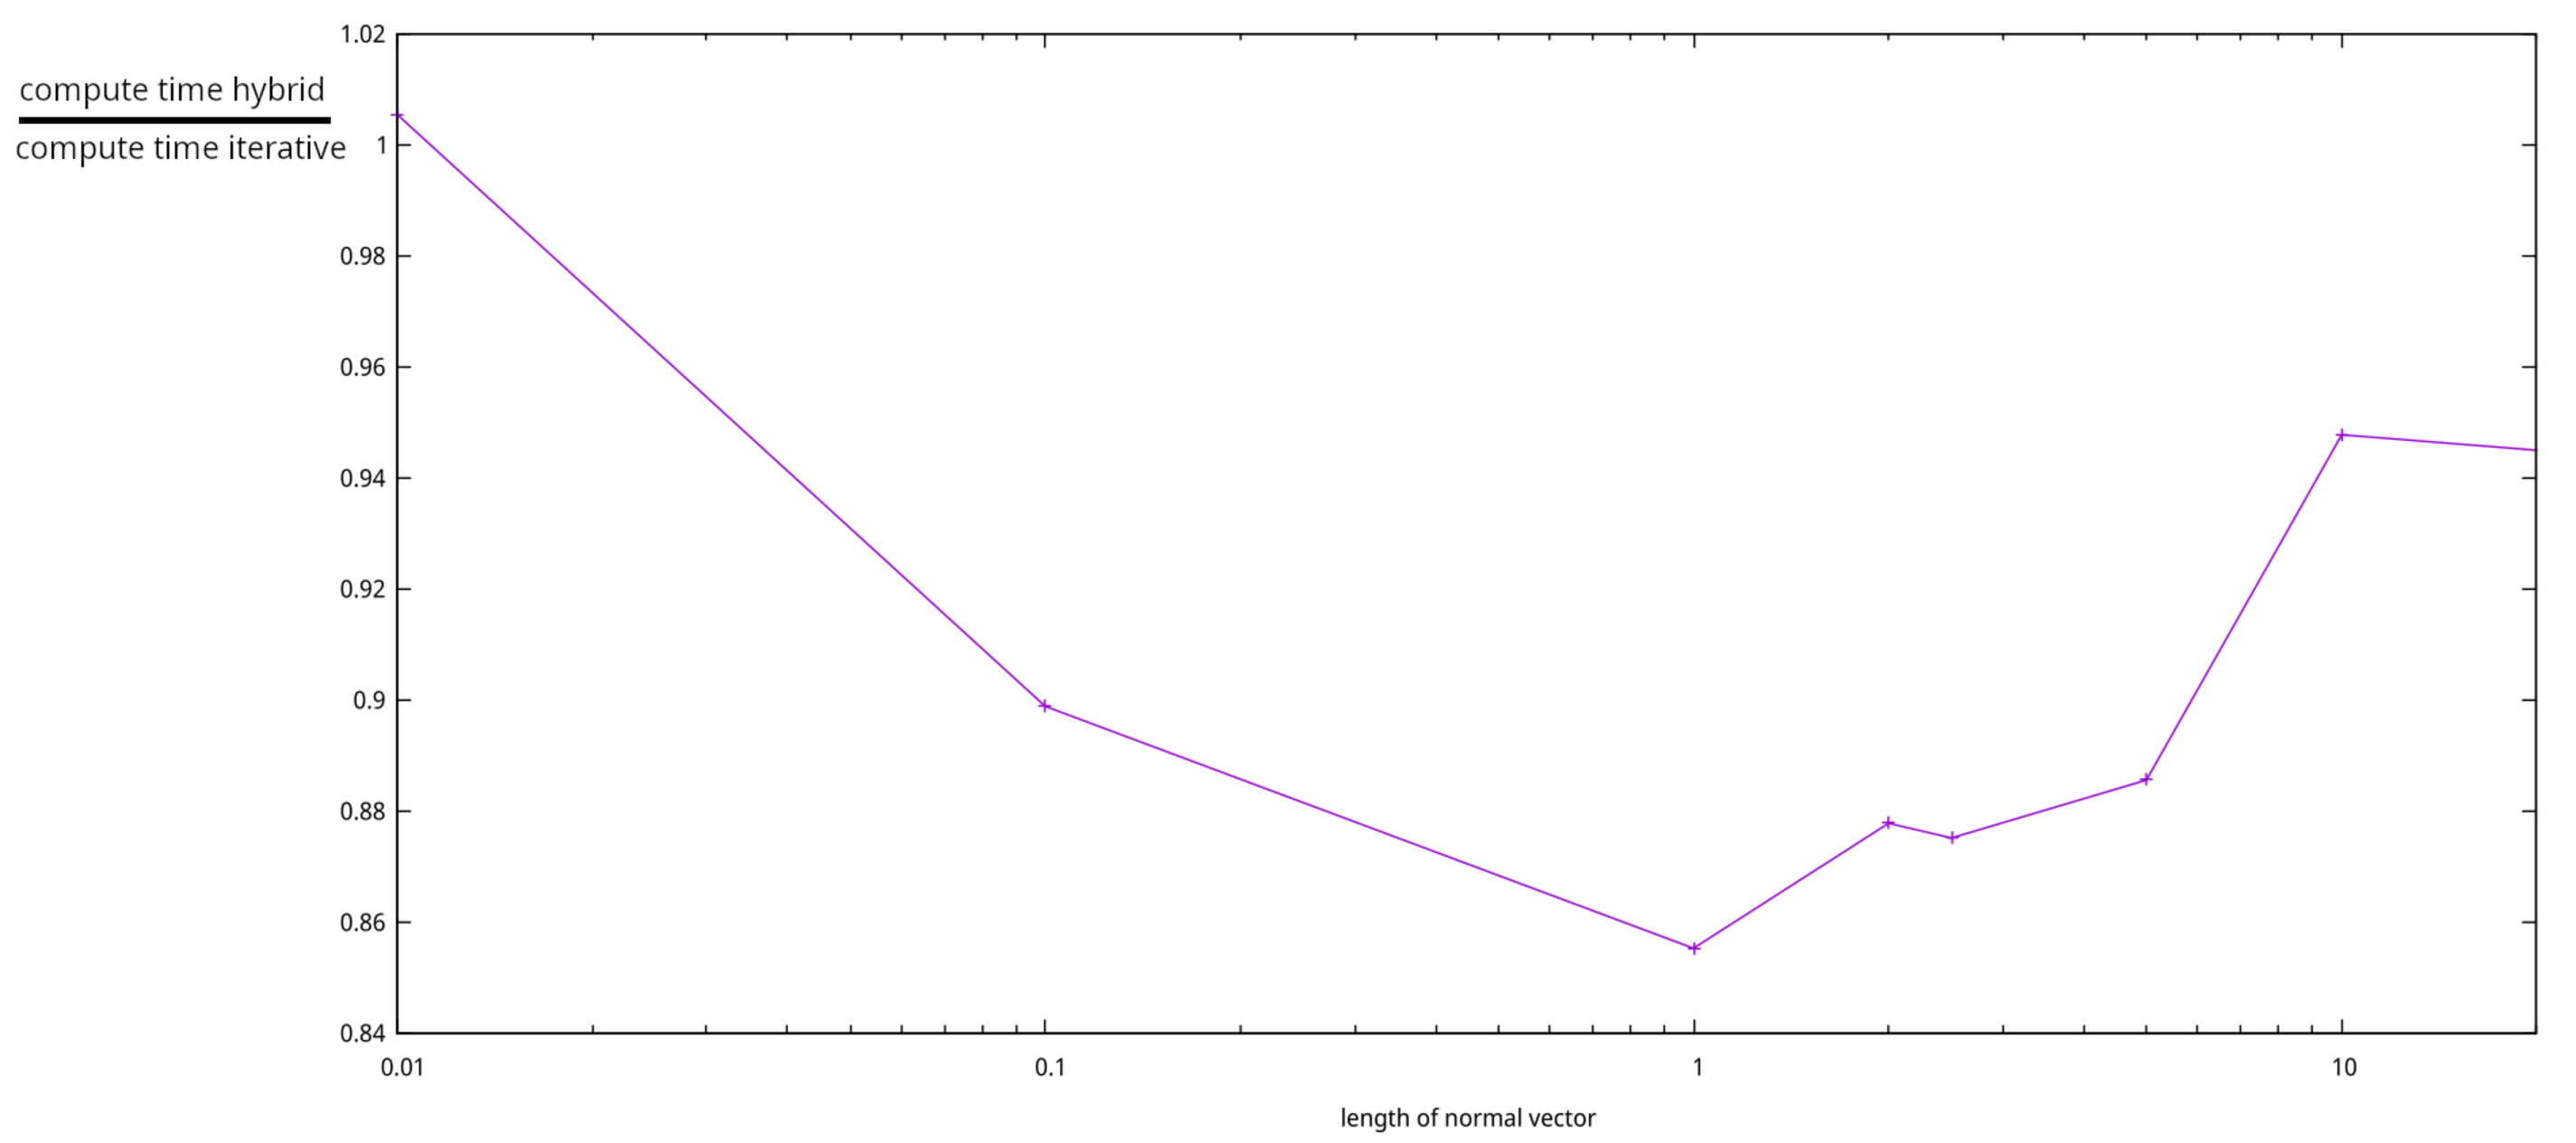
\includegraphics[width=\textwidth]{figures/NormVsTime2.pdf}
	\end{figure}
\end{frame}
\begin{frame}
	First optimization conclusion:\\ Take the normal vector length to be 1 meter.
\end{frame}
\begin{frame}
	\begin{figure}
		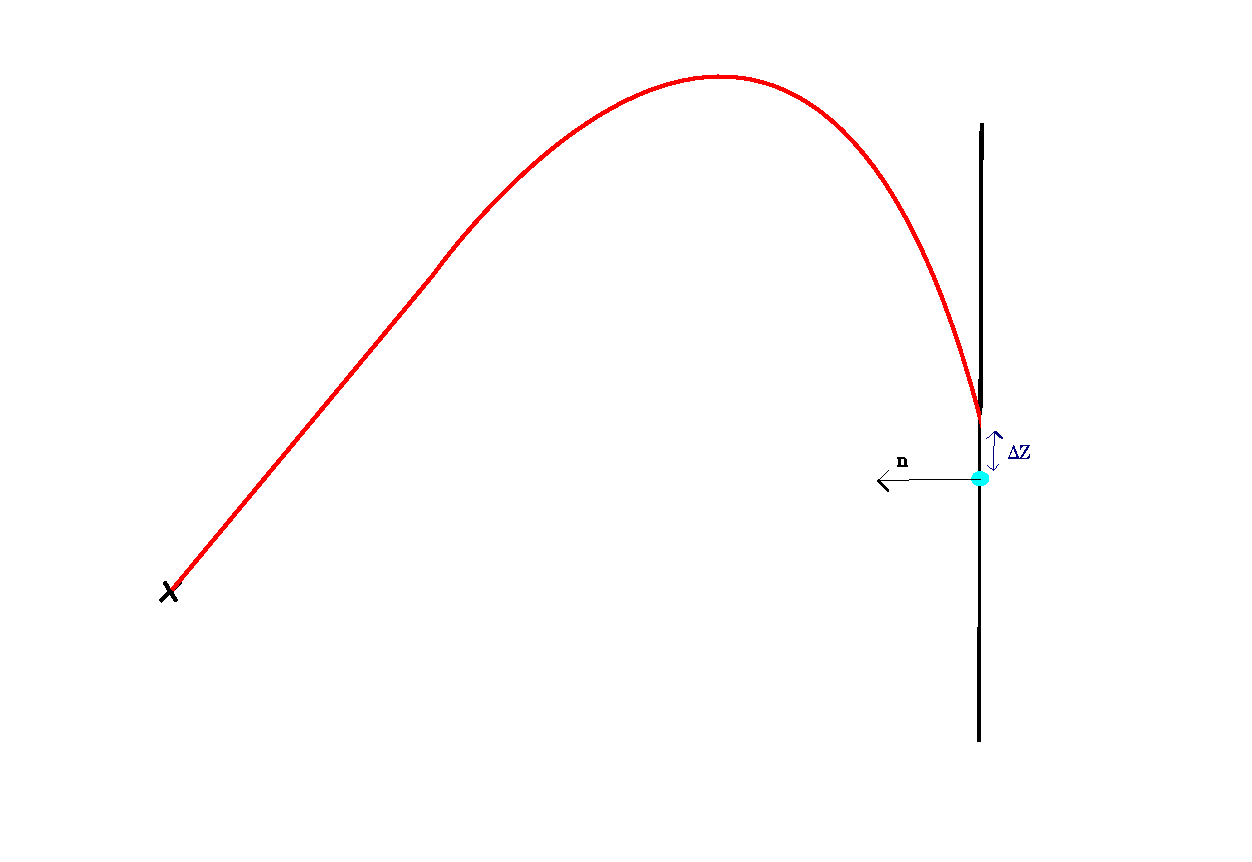
\includegraphics[width=\textwidth]{figures/PrincipleIllu.pdf}
	\end{figure}
\end{frame}
\begin{frame}
	\begin{figure}
		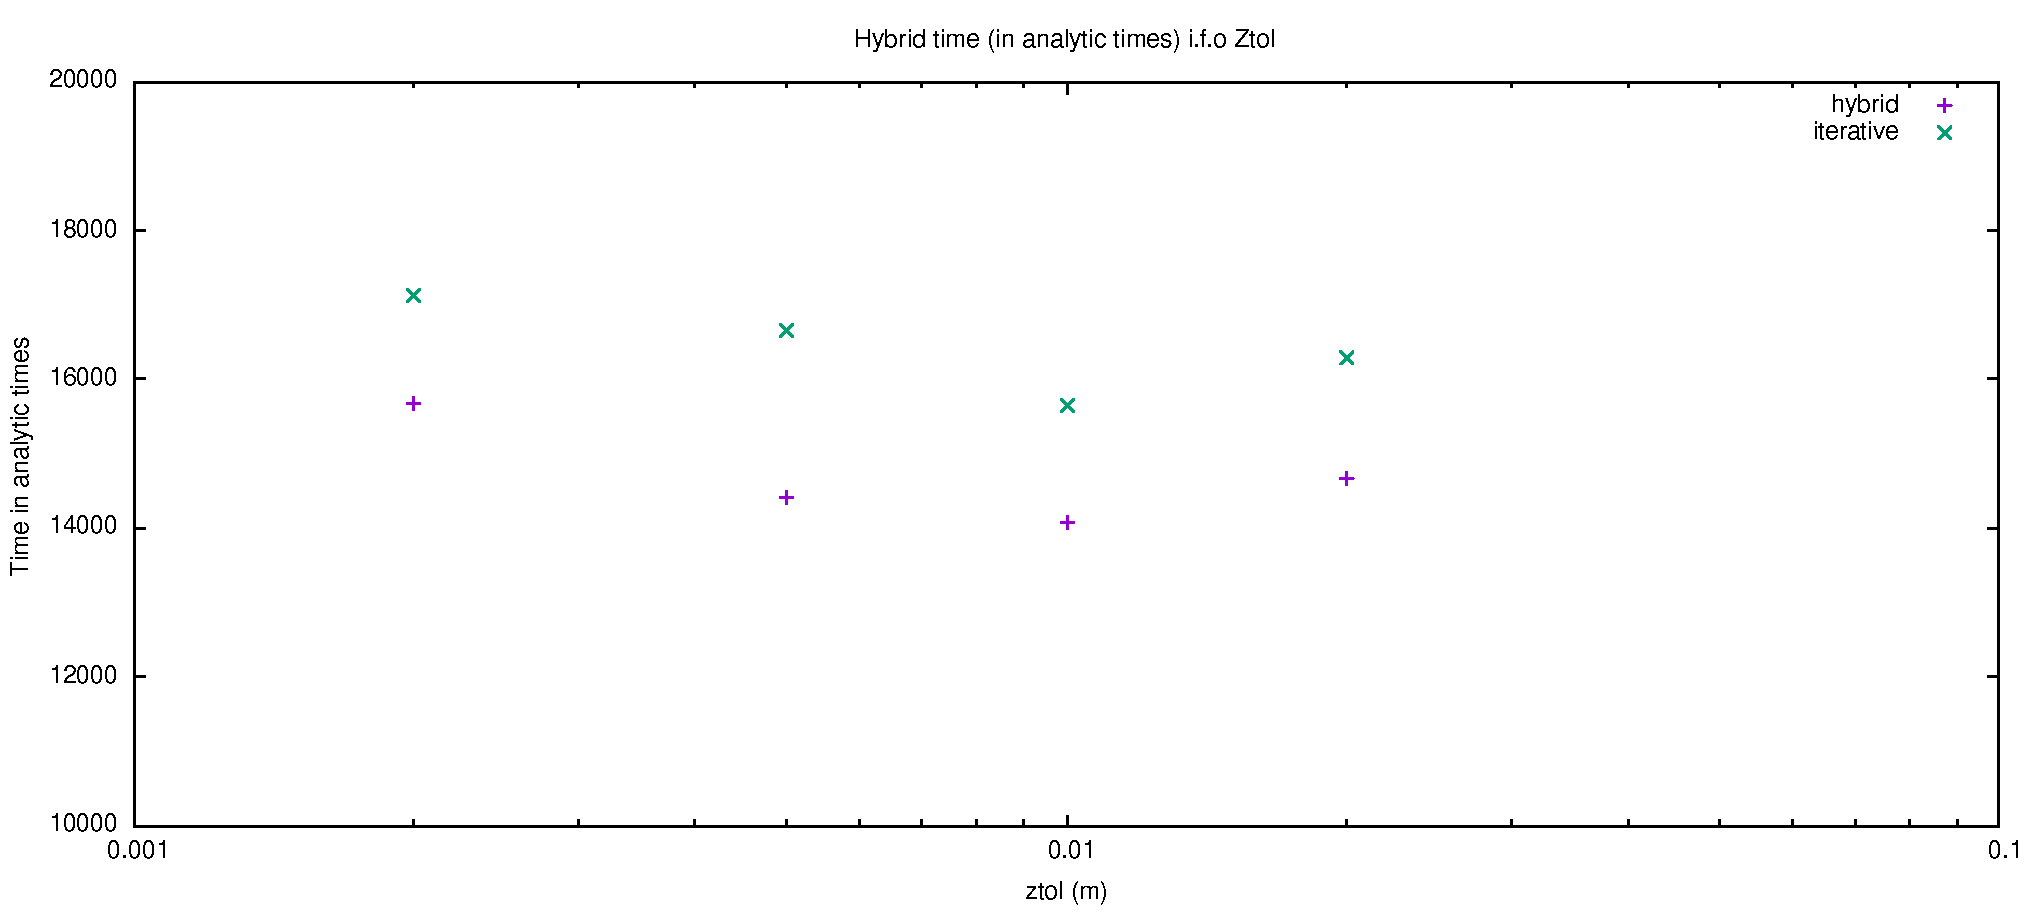
\includegraphics[width=\textwidth]{figures/ZtolVsTime.pdf}
	\end{figure}
\end{frame}
\begin{frame}
	\begin{figure}
		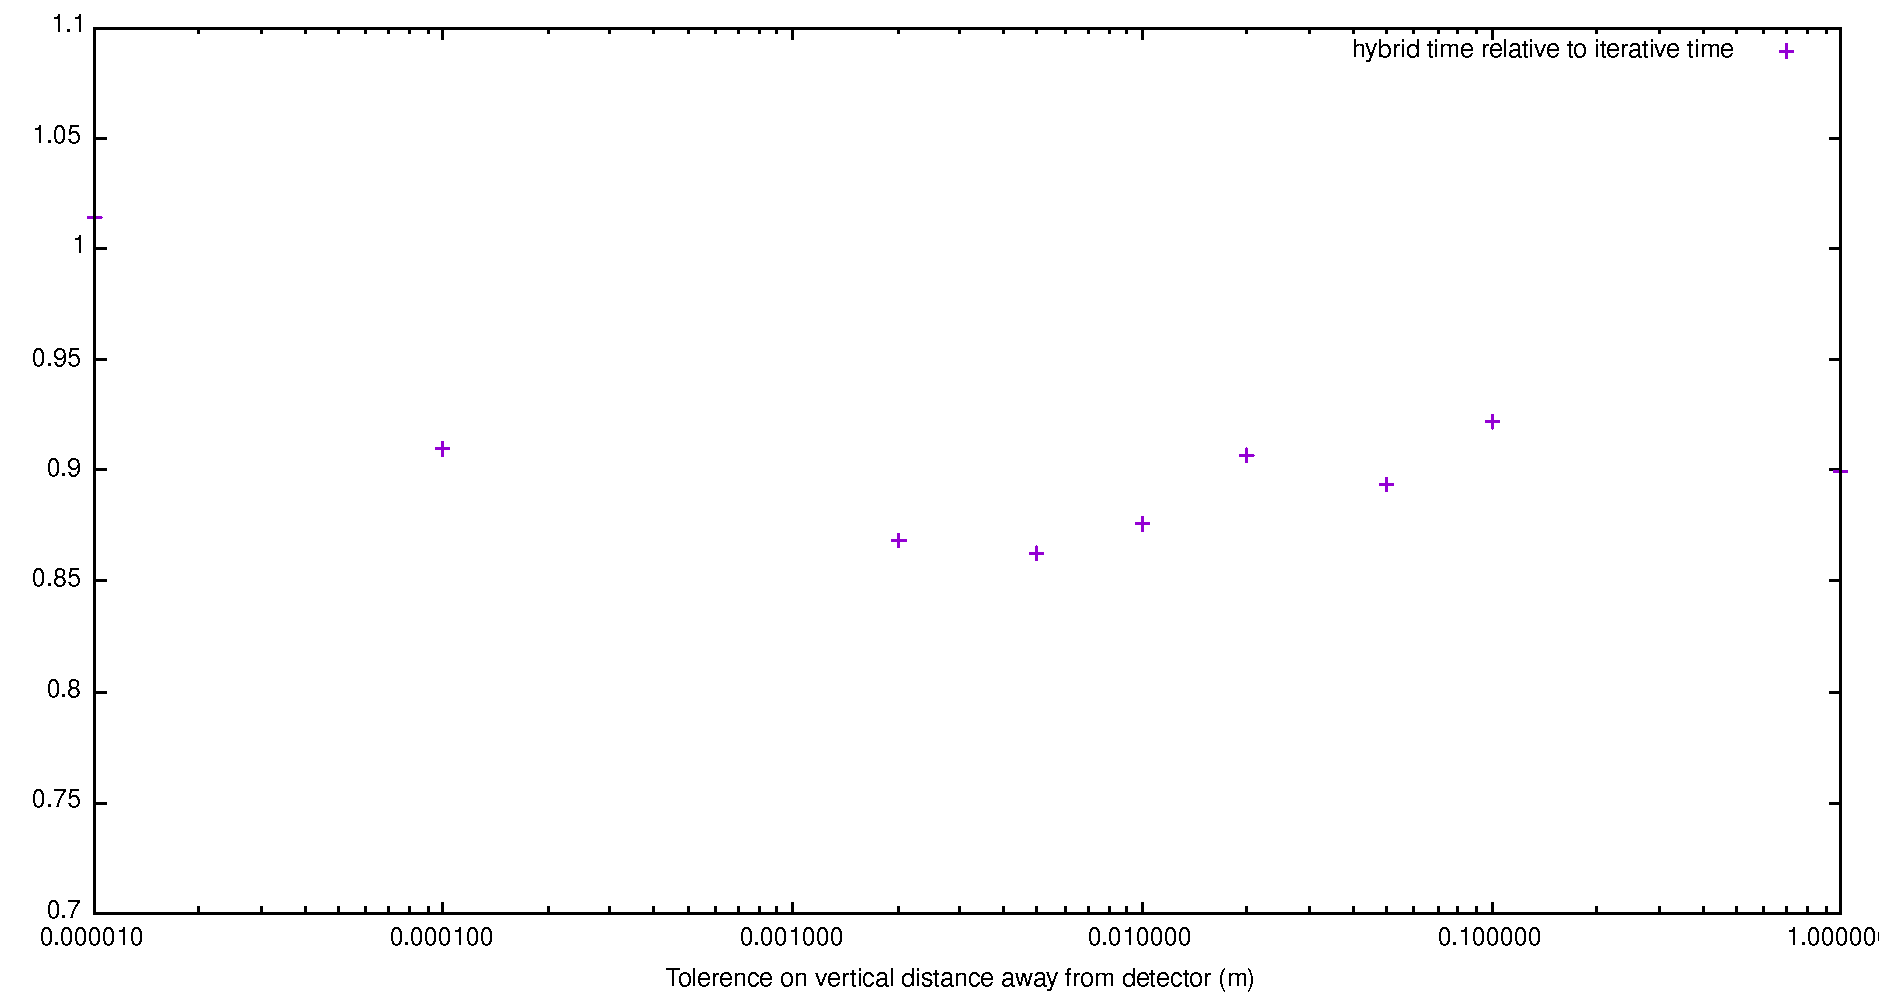
\includegraphics[width=\textwidth]{figures/ZtolVsTime2.pdf}
	\end{figure}
\end{frame}
\begin{frame}
	\begin{figure}
		\begin{minipage}{\textwidth}
			\centering
			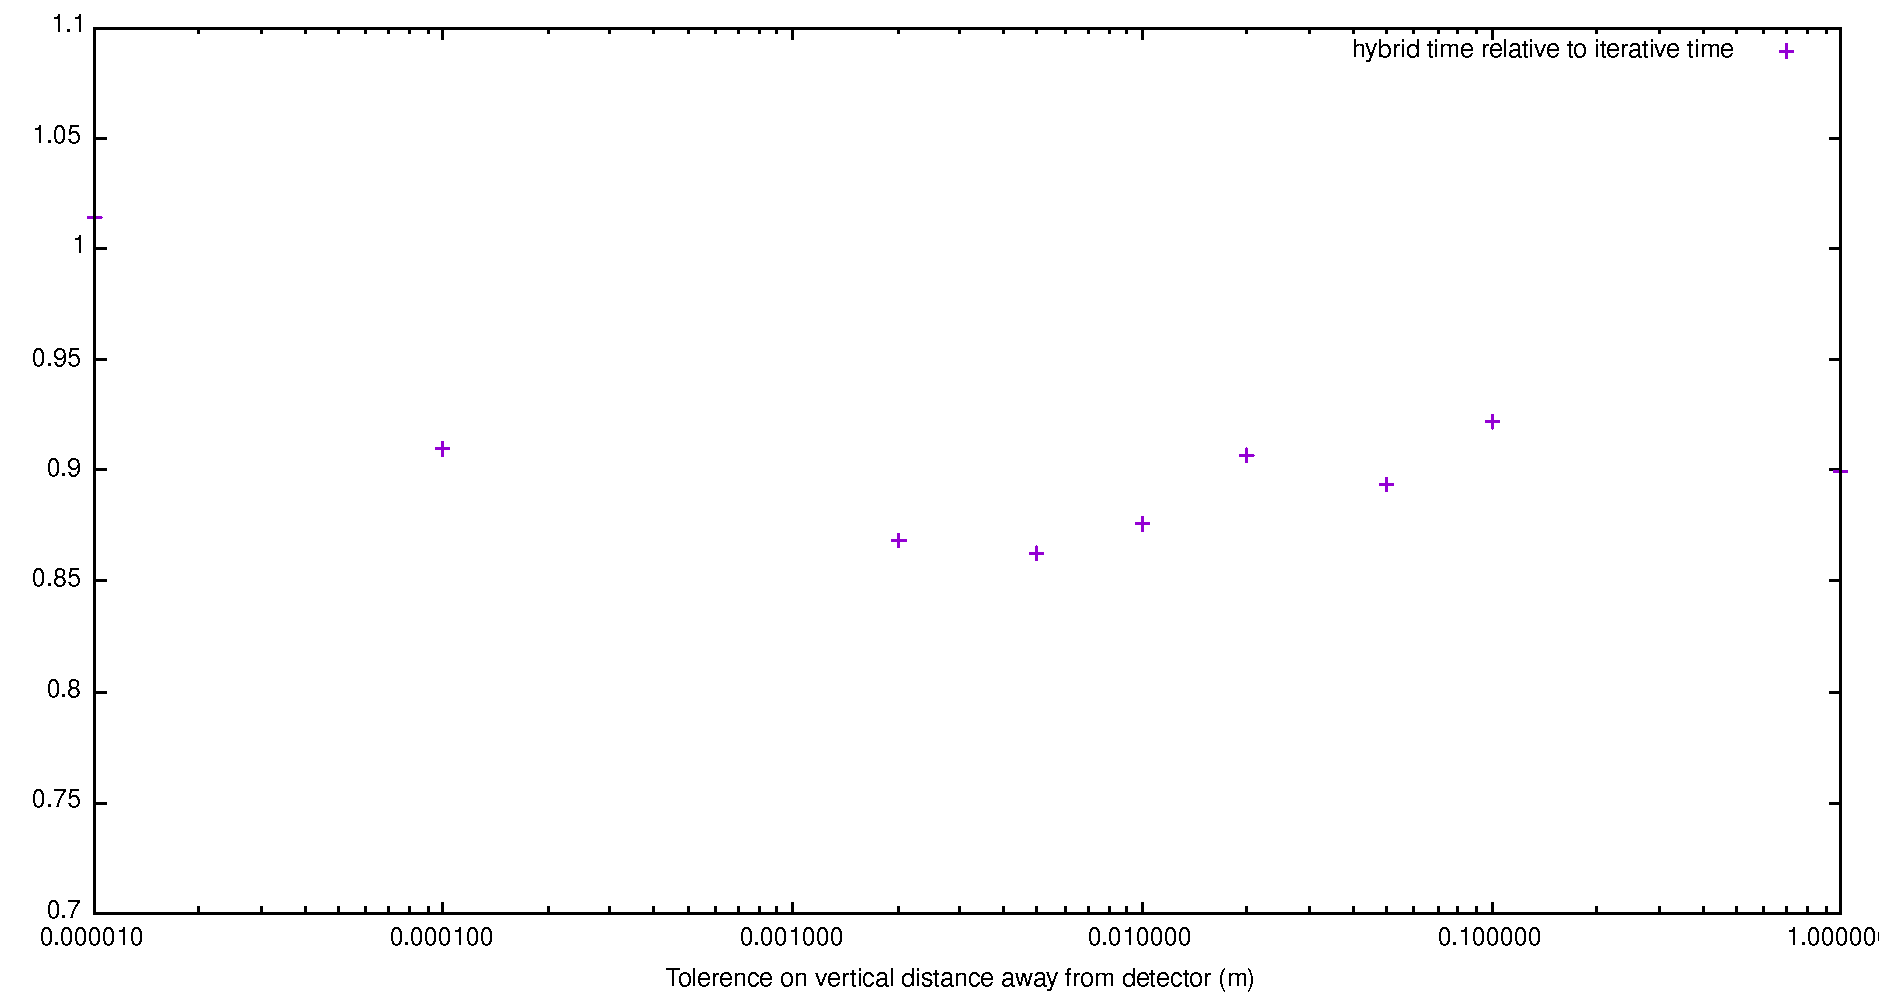
\includegraphics[height=0.45\textheight]{figures/ZtolVsTime2.pdf}
		\end{minipage}
		\begin{minipage}{\textwidth}
			\centering
			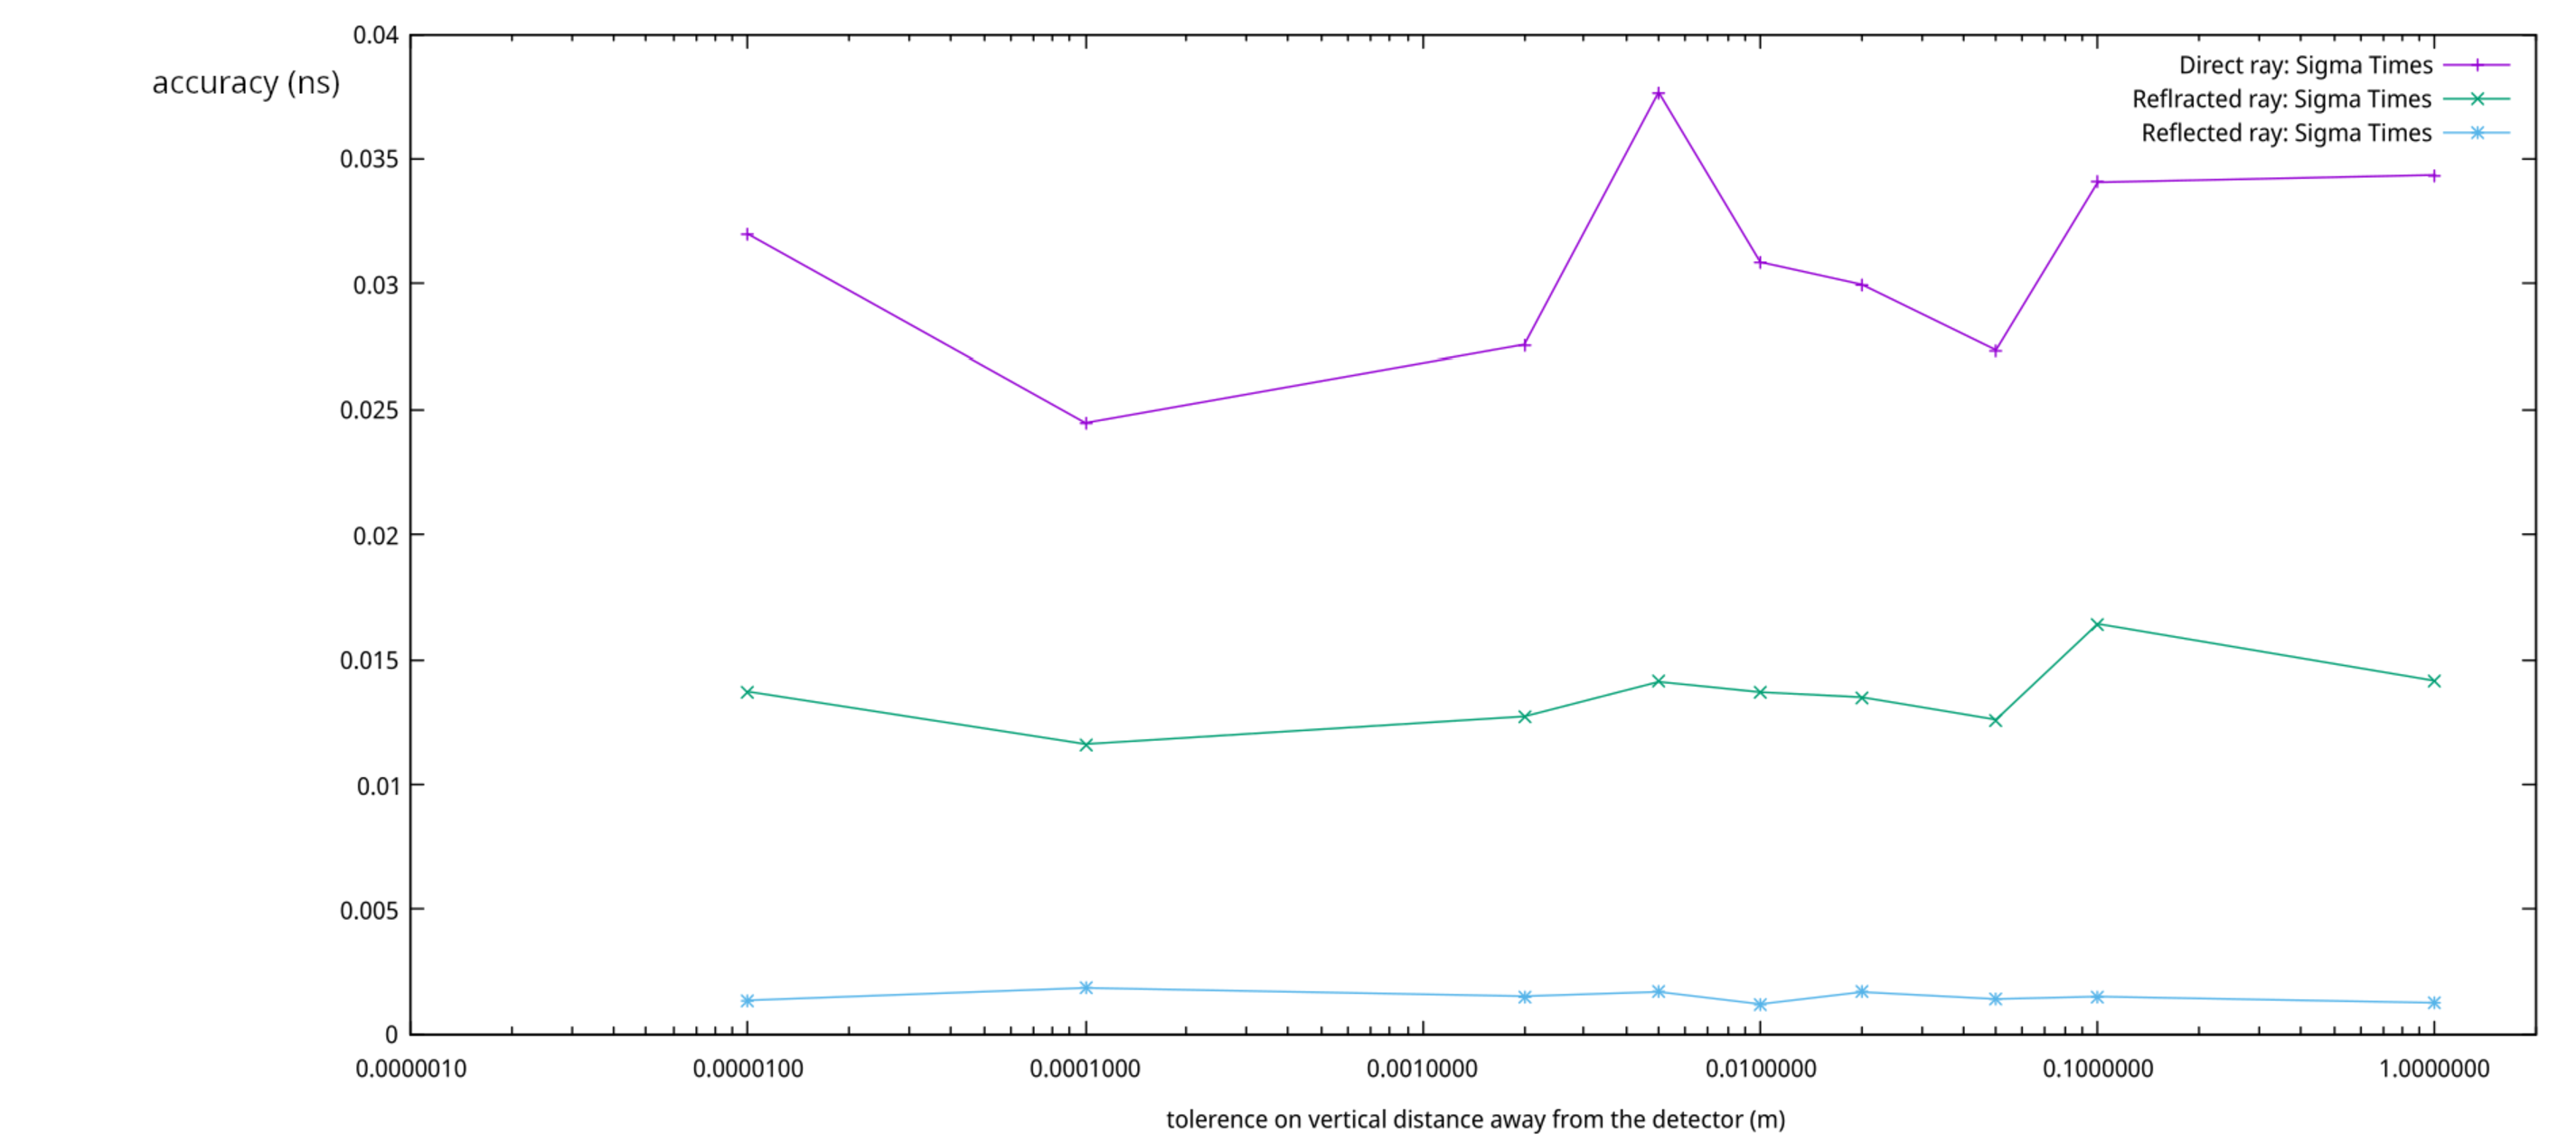
\includegraphics[height=0.45\textheight]{figures/ZtolVsSigmaTime.pdf}
		\end{minipage}
	\end{figure}
\end{frame}
\begin{frame}
	\begin{figure}
		\begin{minipage}{\textwidth}
			\centering
			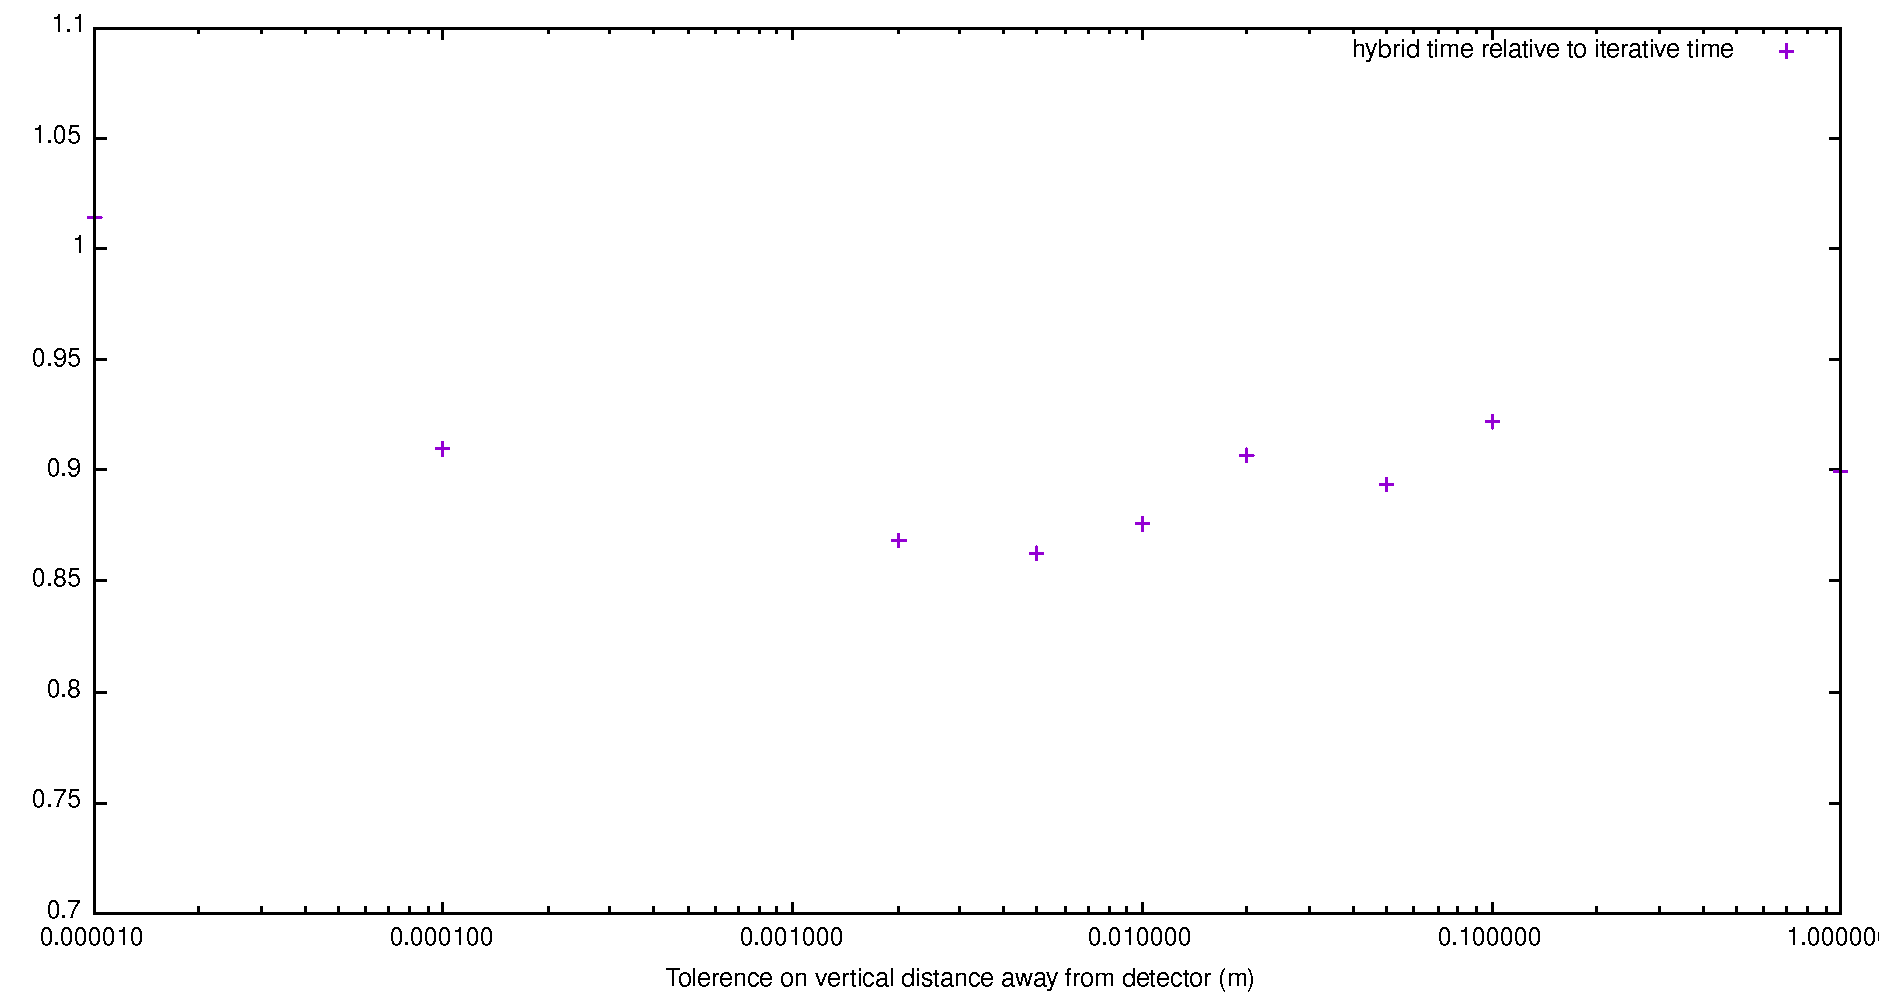
\includegraphics[height=0.45\textheight]{figures/ZtolVsTime2.pdf}
		\end{minipage}
		\begin{minipage}{\textwidth}
			\centering
			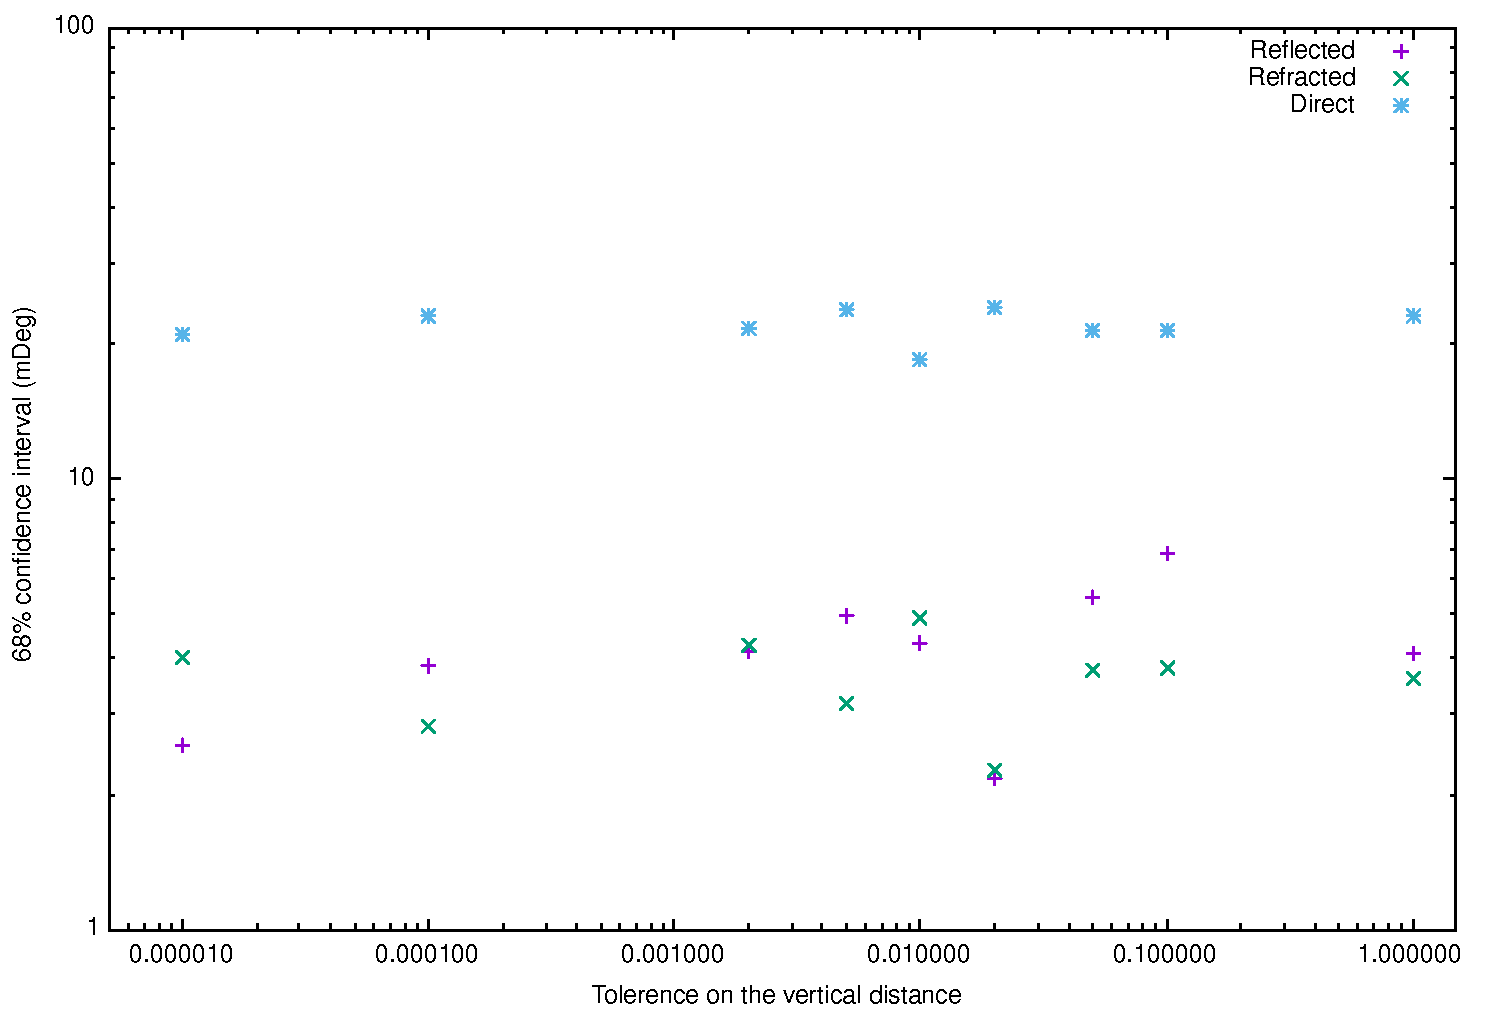
\includegraphics[height=0.45\textheight]{figures/ZtolVsSigmaAZ.pdf}
		\end{minipage}
	\end{figure}
\end{frame}
\begin{frame}
	Second optimization conclusion:\\ Take ztol to be 0.05 m.
\end{frame}
\begin{frame}{Sphere Size \& Step Size}
	\begin{figure}
		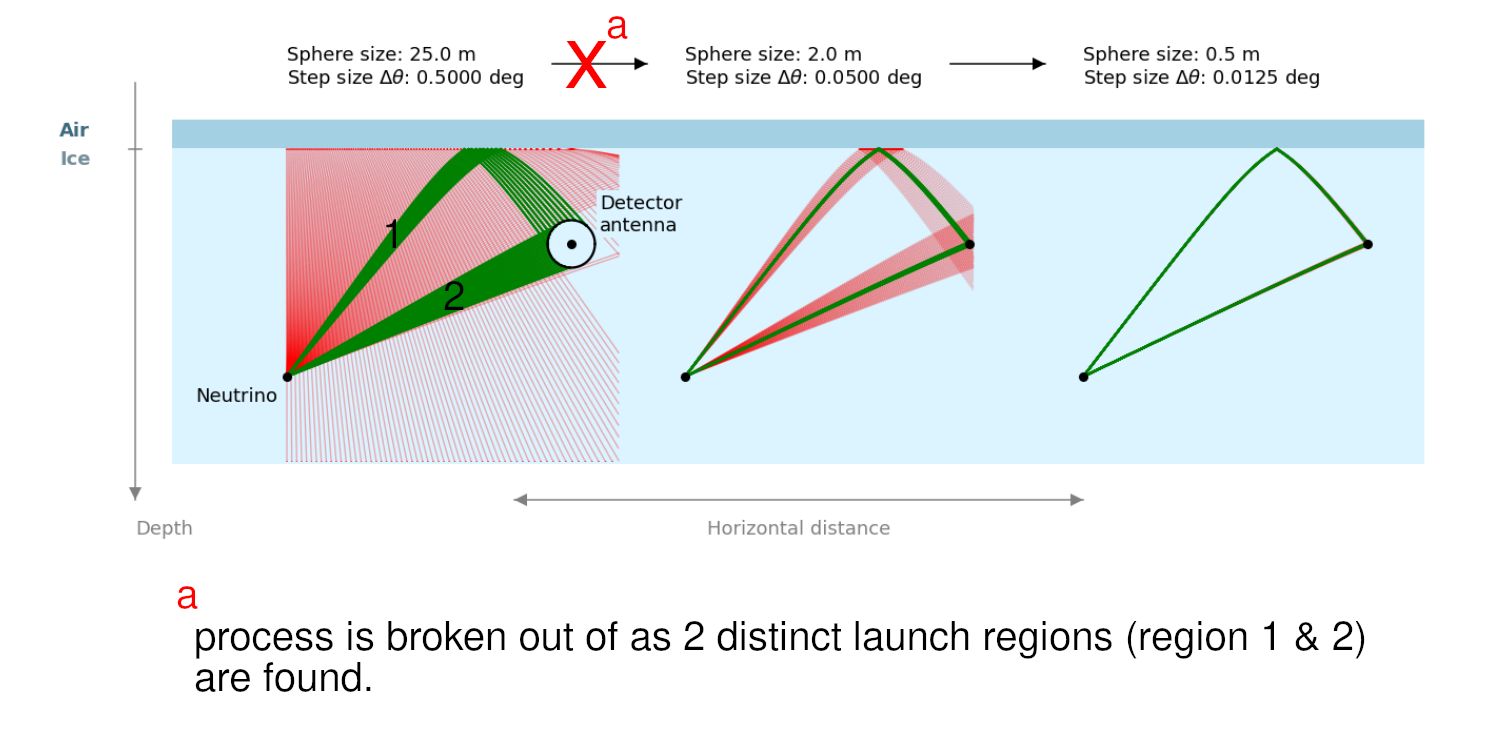
\includegraphics[width=\textwidth]{figures/explanation.png}
	\end{figure}
\end{frame}
\begin{frame}{Sphere Size \& Step Size}
	\begin{figure}
		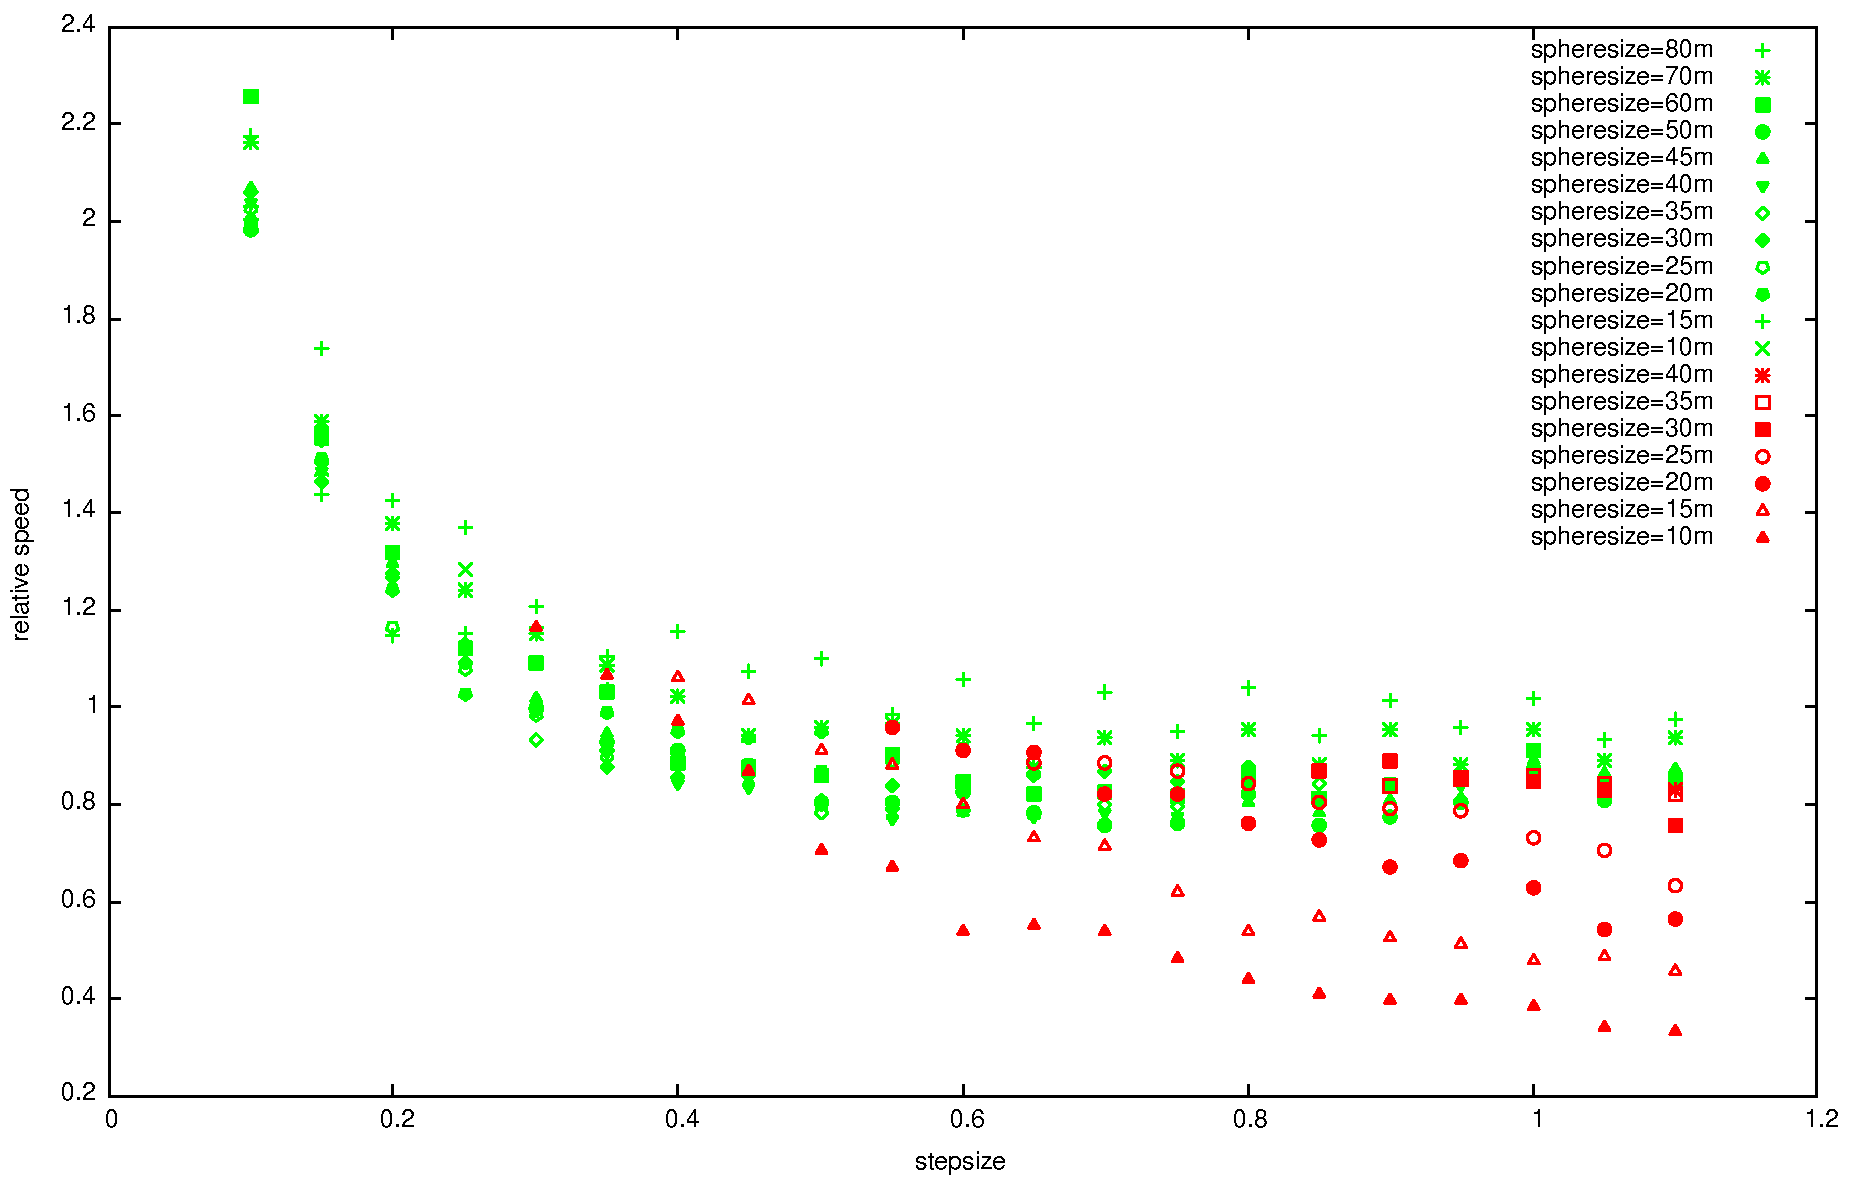
\includegraphics[width=\textwidth]{figures/SphereAndStepAll.pdf}
	\end{figure}
\end{frame}
\begin{frame}{Sphere Size \& Step Size}
	\begin{figure}
		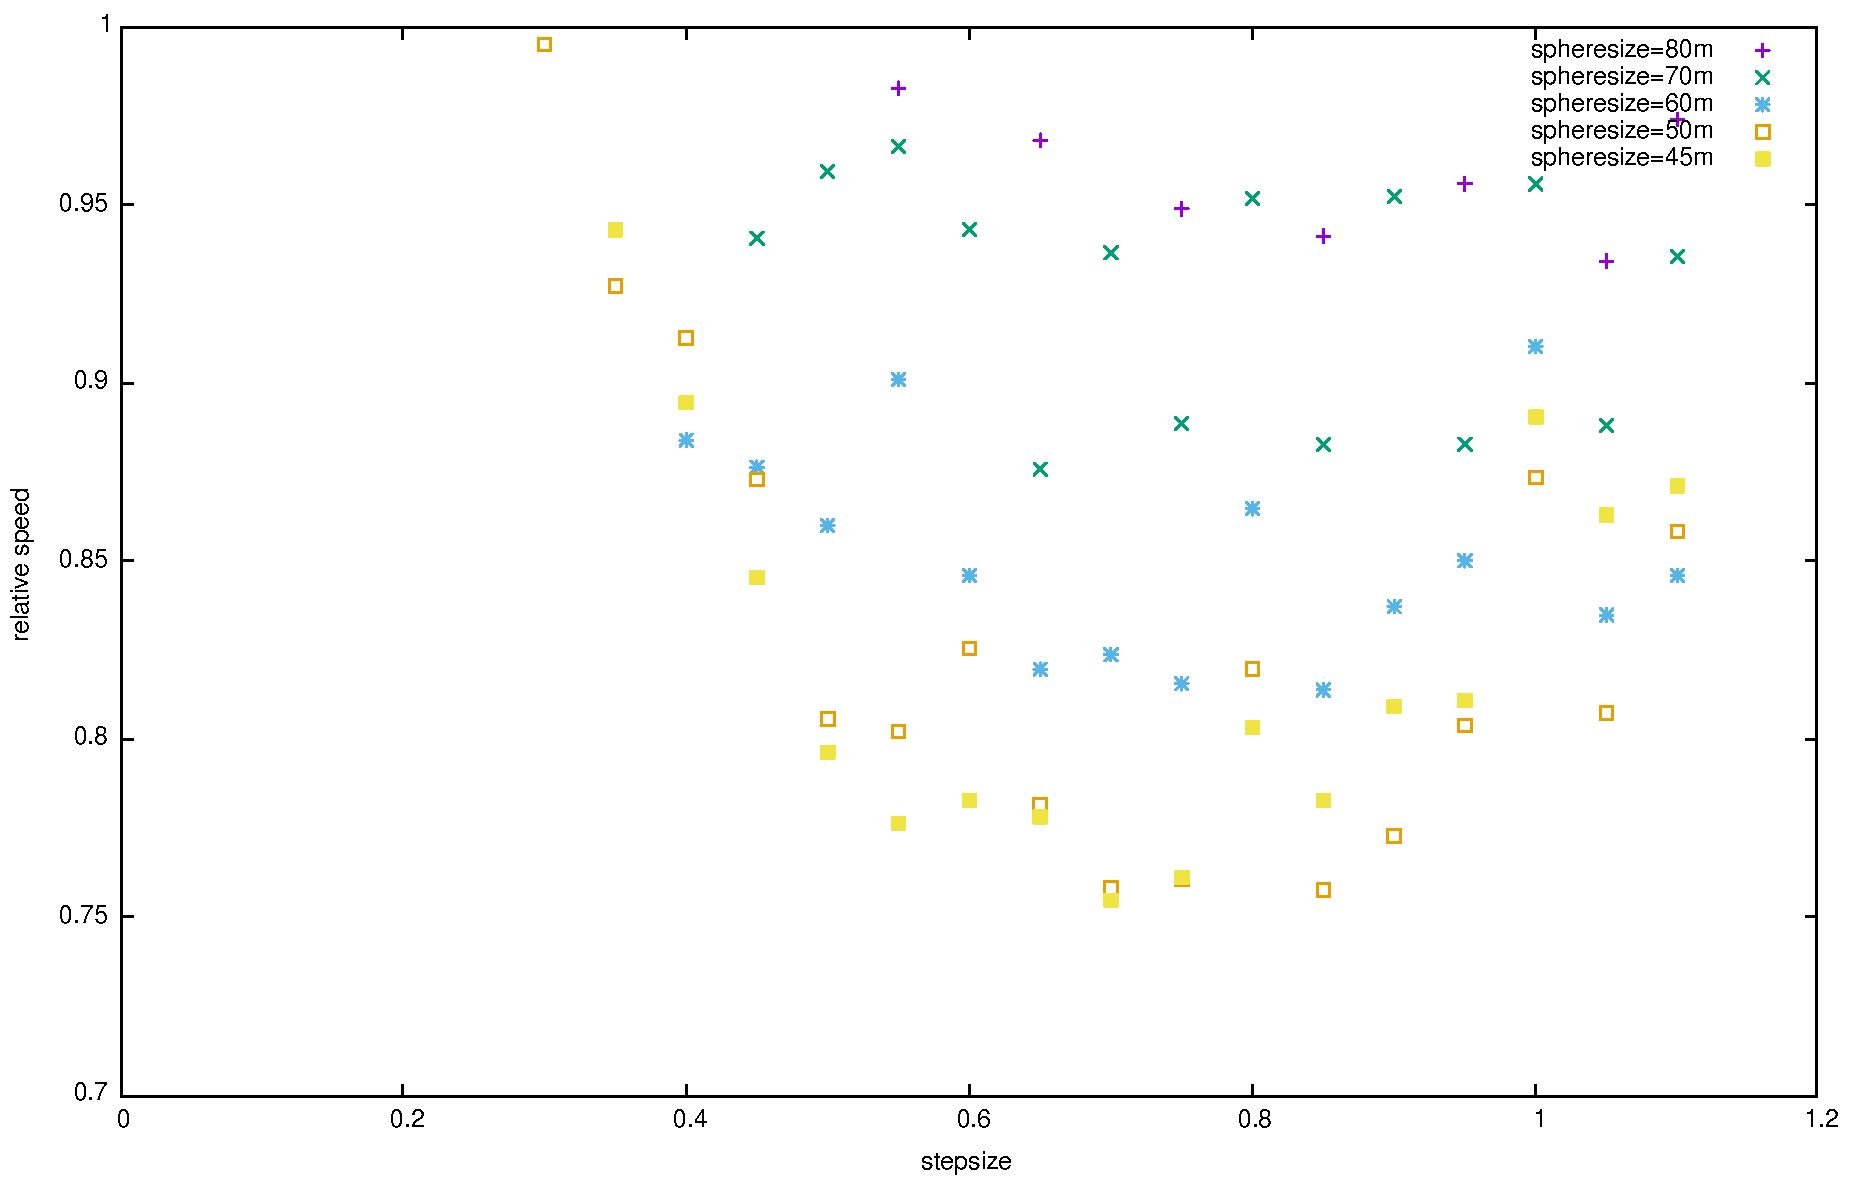
\includegraphics[width=\textwidth]{figures/SphereAndStepFinal.pdf}
	\end{figure}
\end{frame}
\begin{frame}{Final Result}
	\begin{itemize}
		\item norm = 1m
		\item ztol = 0.05m
		\item Sphere size = 45m
		\item step size = 0.7
	\end{itemize}
\end{frame}
\begin{frame}
	\begin{minipage}{0.49\textwidth}
	\begin{figure}
		\centering
		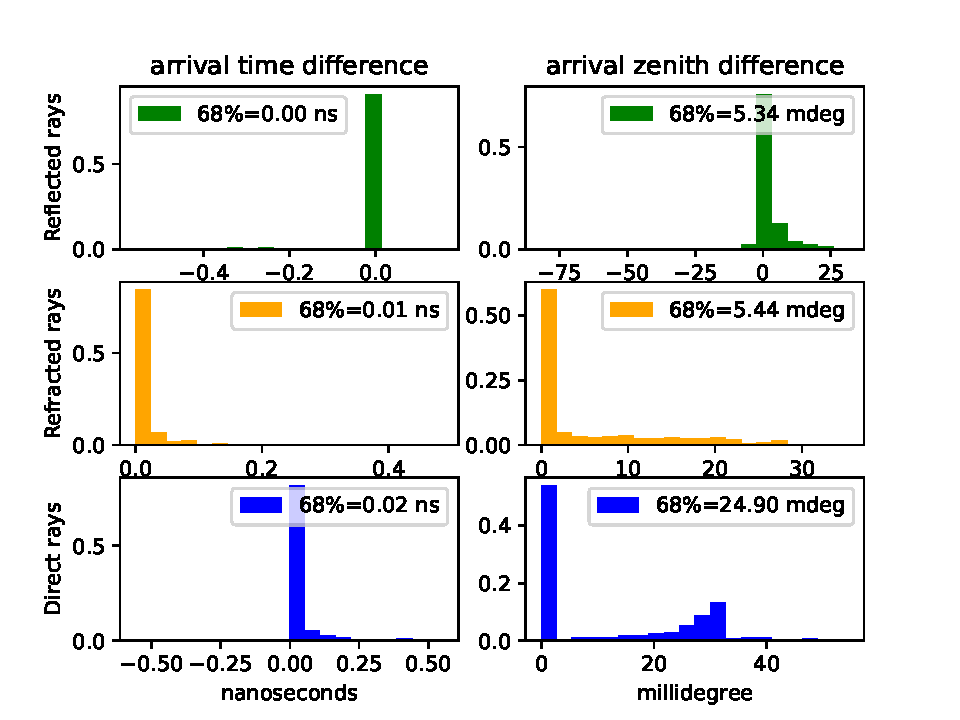
\includegraphics[width=\textwidth]{figures/hybrid_comparison_N_500.pdf}
		\caption{Hybrid}
	\end{figure}
	\end{minipage}
	\begin{minipage}{0.49\textwidth}
	\begin{figure}
		\centering
		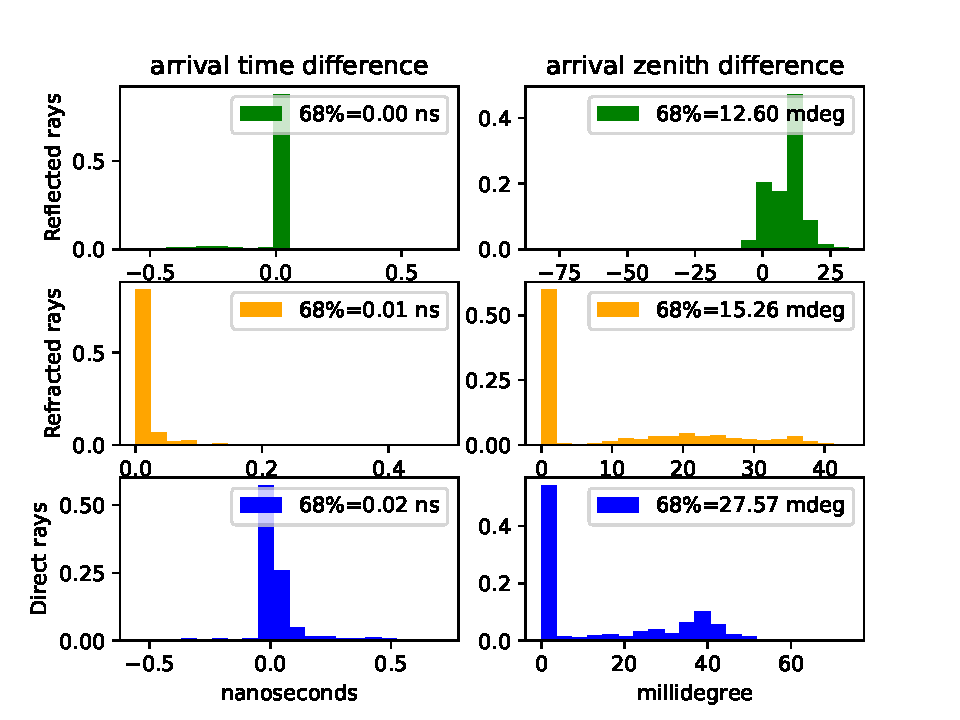
\includegraphics[width=\textwidth]{figures/iterative_comparison_N_500.pdf}
		\caption{Iterative}
	\end{figure}
	\end{minipage}
\end{frame}
\begin{frame}
	\begin{itemize}
		\item iterative :1.627s
		\item hybrid : 1.226s (32.7\% faster)
		\item analytic: 9.719e-05 seconds
	\end{itemize}
\end{frame}
\begin{frame}{What if the same sphere and stepsize?}
	\begin{itemize}
		\item iterative :1.80317s
		\item hybrid : 1.35776s (32.8\% faster)
		\item analytic: 9.8812e-05 seconds
	\end{itemize}\vspace{2cm}
	Exactly the same $\sigma$'s
\end{frame}
\end{document}
